\documentclass [oneside,10pt,a4paper,ngerman,BCOR10mm,headsepline,parindent,final]{scrartcl}

    \usepackage[breakable]{tcolorbox}
    \usepackage{parskip} % Stop auto-indenting (to mimic markdown behaviour)
    

    % Basic figure setup, for now with no caption control since it's done
    % automatically by Pandoc (which extracts ![](path) syntax from Markdown).
    \usepackage{graphicx}
    % Maintain compatibility with old templates. Remove in nbconvert 6.0
    % \let\Oldincludegraphics\includegraphics
    % Ensure that by default, figures have no caption (until we provide a
    % proper Figure object with a Caption API and a way to capture that
    % in the conversion process - todo).
    % \usepackage{caption}
    % \DeclareCaptionFormat{nocaption}{}
    % \captionsetup{format=nocaption,aboveskip=0pt,belowskip=0pt}

    \usepackage{float}
    \floatplacement{figure}{H} % forces figures to be placed at the correct location
    \usepackage{xcolor} % Allow colors to be defined
    \usepackage{enumerate} % Needed for markdown enumerations to work
    \usepackage{geometry} % Used to adjust the document margins
    \usepackage{amsmath} % Equations
    \usepackage{amssymb} % Equations
    \usepackage{textcomp} % defines textquotesingle
    % Hack from http://tex.stackexchange.com/a/47451/13684:
    \AtBeginDocument{%
        \def\PYZsq{\textquotesingle}% Upright quotes in Pygmentized code
    }
    \usepackage{upquote} % Upright quotes for verbatim code
    \usepackage{eurosym} % defines \euro

    \usepackage{iftex}
    \ifPDFTeX
        \usepackage[T1]{fontenc}
        \usepackage[utf8]{inputenc}
    \else
        \usepackage{fontspec}
        \usepackage{unicode-math}
    \fi

    \usepackage{fancyvrb} % verbatim replacement that allows latex
    \usepackage{grffile} % extends the file name processing of package graphics 
                         % to support a larger range
    \makeatletter % fix for old versions of grffile with XeLaTeX
    \@ifpackagelater{grffile}{2019/11/01}
    {
      % Do nothing on new versions
    }
    {
      \def\Gread@@xetex#1{%
        \IfFileExists{"\Gin@base".bb}%
        {\Gread@eps{\Gin@base.bb}}%
        {\Gread@@xetex@aux#1}%
      }
    }
    \makeatother
    \usepackage[Export]{adjustbox} % Used to constrain images to a maximum size
    \adjustboxset{max size={0.9\linewidth}{0.9\paperheight}}

    % The hyperref package gives us a pdf with properly built
    % internal navigation ('pdf bookmarks' for the table of contents,
    % internal cross-reference links, web links for URLs, etc.)
    \usepackage{hyperref}
    % The default LaTeX title has an obnoxious amount of whitespace. By default,
    % titling removes some of it. It also provides customization options.
    \usepackage{titling}
    \usepackage{longtable} % longtable support required by pandoc >1.10
    \usepackage{booktabs}  % table support for pandoc > 1.12.2
    \usepackage{array}     % table support for pandoc >= 2.11.3
    \usepackage{calc}      % table minipage width calculation for pandoc >= 2.11.1
    \usepackage[inline]{enumitem} % IRkernel/repr support (it uses the enumerate* environment)
    \usepackage[normalem]{ulem} % ulem is needed to support strikethroughs (\sout)
                                % normalem makes italics be italics, not underlines
    \usepackage{mathrsfs}
    
    % Using fancy headers and footers
    \usepackage{fancyhdr}
    
    % Used for entering author names and their affiliations
    \usepackage[affil-it]{authblk}
    
    % Use bibliography% and configure it
    \usepackage[babel,german=quotes]{csquotes}
    \usepackage[backend=biber,style=authoryear,backref=true]{biblatex}
    \bibliography{literature/notebook.bib}
    \usepackage{url}                    %Output of nicely formatted Internet addresses
    \setcounter{biburllcpenalty}{7000}  %Setting for counter to wrap URLs in literature references
    \setcounter{biburlucpenalty}{8000}  %ditto



    
    % Colors for the hyperref package
    \definecolor{urlcolor}{rgb}{0,.145,.698}
    \definecolor{linkcolor}{rgb}{.71,0.21,0.01}
    \definecolor{citecolor}{rgb}{.12,.54,.11}

    % ANSI colors
    \definecolor{ansi-black}{HTML}{3E424D}
    \definecolor{ansi-black-intense}{HTML}{282C36}
    \definecolor{ansi-red}{HTML}{E75C58}
    \definecolor{ansi-red-intense}{HTML}{B22B31}
    \definecolor{ansi-green}{HTML}{00A250}
    \definecolor{ansi-green-intense}{HTML}{007427}
    \definecolor{ansi-yellow}{HTML}{DDB62B}
    \definecolor{ansi-yellow-intense}{HTML}{B27D12}
    \definecolor{ansi-blue}{HTML}{208FFB}
    \definecolor{ansi-blue-intense}{HTML}{0065CA}
    \definecolor{ansi-magenta}{HTML}{D160C4}
    \definecolor{ansi-magenta-intense}{HTML}{A03196}
    \definecolor{ansi-cyan}{HTML}{60C6C8}
    \definecolor{ansi-cyan-intense}{HTML}{258F8F}
    \definecolor{ansi-white}{HTML}{C5C1B4}
    \definecolor{ansi-white-intense}{HTML}{A1A6B2}
    \definecolor{ansi-default-inverse-fg}{HTML}{FFFFFF}
    \definecolor{ansi-default-inverse-bg}{HTML}{000000}

    % common color for the border for error outputs.
    \definecolor{outerrorbackground}{HTML}{FFDFDF}

    % commands and environments needed by pandoc snippets
    % extracted from the output of `pandoc -s`
    \providecommand{\tightlist}{%
      \setlength{\itemsep}{0pt}\setlength{\parskip}{0pt}}
    \DefineVerbatimEnvironment{Highlighting}{Verbatim}{commandchars=\\\{\}}
    % Add ',fontsize=\small' for more characters per line
    \newenvironment{Shaded}{}{}
    \newcommand{\KeywordTok}[1]{\textcolor[rgb]{0.00,0.44,0.13}{\textbf{{#1}}}}
    \newcommand{\DataTypeTok}[1]{\textcolor[rgb]{0.56,0.13,0.00}{{#1}}}
    \newcommand{\DecValTok}[1]{\textcolor[rgb]{0.25,0.63,0.44}{{#1}}}
    \newcommand{\BaseNTok}[1]{\textcolor[rgb]{0.25,0.63,0.44}{{#1}}}
    \newcommand{\FloatTok}[1]{\textcolor[rgb]{0.25,0.63,0.44}{{#1}}}
    \newcommand{\CharTok}[1]{\textcolor[rgb]{0.25,0.44,0.63}{{#1}}}
    \newcommand{\StringTok}[1]{\textcolor[rgb]{0.25,0.44,0.63}{{#1}}}
    \newcommand{\CommentTok}[1]{\textcolor[rgb]{0.38,0.63,0.69}{\textit{{#1}}}}
    \newcommand{\OtherTok}[1]{\textcolor[rgb]{0.00,0.44,0.13}{{#1}}}
    \newcommand{\AlertTok}[1]{\textcolor[rgb]{1.00,0.00,0.00}{\textbf{{#1}}}}
    \newcommand{\FunctionTok}[1]{\textcolor[rgb]{0.02,0.16,0.49}{{#1}}}
    \newcommand{\RegionMarkerTok}[1]{{#1}}
    \newcommand{\ErrorTok}[1]{\textcolor[rgb]{1.00,0.00,0.00}{\textbf{{#1}}}}
    \newcommand{\NormalTok}[1]{{#1}}
    
    % Additional commands for more recent versions of Pandoc
    \newcommand{\ConstantTok}[1]{\textcolor[rgb]{0.53,0.00,0.00}{{#1}}}
    \newcommand{\SpecialCharTok}[1]{\textcolor[rgb]{0.25,0.44,0.63}{{#1}}}
    \newcommand{\VerbatimStringTok}[1]{\textcolor[rgb]{0.25,0.44,0.63}{{#1}}}
    \newcommand{\SpecialStringTok}[1]{\textcolor[rgb]{0.73,0.40,0.53}{{#1}}}
    \newcommand{\ImportTok}[1]{{#1}}
    \newcommand{\DocumentationTok}[1]{\textcolor[rgb]{0.73,0.13,0.13}{\textit{{#1}}}}
    \newcommand{\AnnotationTok}[1]{\textcolor[rgb]{0.38,0.63,0.69}{\textbf{\textit{{#1}}}}}
    \newcommand{\CommentVarTok}[1]{\textcolor[rgb]{0.38,0.63,0.69}{\textbf{\textit{{#1}}}}}
    \newcommand{\VariableTok}[1]{\textcolor[rgb]{0.10,0.09,0.49}{{#1}}}
    \newcommand{\ControlFlowTok}[1]{\textcolor[rgb]{0.00,0.44,0.13}{\textbf{{#1}}}}
    \newcommand{\OperatorTok}[1]{\textcolor[rgb]{0.40,0.40,0.40}{{#1}}}
    \newcommand{\BuiltInTok}[1]{{#1}}
    \newcommand{\ExtensionTok}[1]{{#1}}
    \newcommand{\PreprocessorTok}[1]{\textcolor[rgb]{0.74,0.48,0.00}{{#1}}}
    \newcommand{\AttributeTok}[1]{\textcolor[rgb]{0.49,0.56,0.16}{{#1}}}
    \newcommand{\InformationTok}[1]{\textcolor[rgb]{0.38,0.63,0.69}{\textbf{\textit{{#1}}}}}
    \newcommand{\WarningTok}[1]{\textcolor[rgb]{0.38,0.63,0.69}{\textbf{\textit{{#1}}}}}
    
    
    % Define a nice break command that doesn't care if a line doesn't already
    % exist.
    \def\br{\hspace*{\fill} \\* }
    % Math Jax compatibility definitions
    \def\gt{>}
    \def\lt{<}
    \let\Oldtex\TeX
    \let\Oldlatex\LaTeX
    \renewcommand{\TeX}{\textrm{\Oldtex}}
    \renewcommand{\LaTeX}{\textrm{\Oldlatex}}
    % Document parameters
    % Document title
    \title{\textbf{\textsf{Preparing raw CSV input data from survey for analytical hierarchy process (AHP)}}}
\author[1]{Bj\"orn Kasper (\href{mailto:kasper.bjoern@bgetem.de}{kasper.bjoern@bgetem.de})}
\affil[1]{Berufsgenossenschaft Energie Textil Elektro Medienerzeugnisse}
\author[2]{Henriette John (\href{mailto:h.john@ioer.de}{h.john@ioer.de})}
\affil[2]{Leibniz Institute of Ecological Urban and Regional Development}\date{\today; version 0.1 (pre-release)}


    
    
    
    
    
% Pygments definitions
\makeatletter
\def\PY@reset{\let\PY@it=\relax \let\PY@bf=\relax%
    \let\PY@ul=\relax \let\PY@tc=\relax%
    \let\PY@bc=\relax \let\PY@ff=\relax}
\def\PY@tok#1{\csname PY@tok@#1\endcsname}
\def\PY@toks#1+{\ifx\relax#1\empty\else%
    \PY@tok{#1}\expandafter\PY@toks\fi}
\def\PY@do#1{\PY@bc{\PY@tc{\PY@ul{%
    \PY@it{\PY@bf{\PY@ff{#1}}}}}}}
\def\PY#1#2{\PY@reset\PY@toks#1+\relax+\PY@do{#2}}

\@namedef{PY@tok@w}{\def\PY@tc##1{\textcolor[rgb]{0.73,0.73,0.73}{##1}}}
\@namedef{PY@tok@c}{\let\PY@it=\textit\def\PY@tc##1{\textcolor[rgb]{0.24,0.48,0.48}{##1}}}
\@namedef{PY@tok@cp}{\def\PY@tc##1{\textcolor[rgb]{0.61,0.40,0.00}{##1}}}
\@namedef{PY@tok@k}{\let\PY@bf=\textbf\def\PY@tc##1{\textcolor[rgb]{0.00,0.50,0.00}{##1}}}
\@namedef{PY@tok@kp}{\def\PY@tc##1{\textcolor[rgb]{0.00,0.50,0.00}{##1}}}
\@namedef{PY@tok@kt}{\def\PY@tc##1{\textcolor[rgb]{0.69,0.00,0.25}{##1}}}
\@namedef{PY@tok@o}{\def\PY@tc##1{\textcolor[rgb]{0.40,0.40,0.40}{##1}}}
\@namedef{PY@tok@ow}{\let\PY@bf=\textbf\def\PY@tc##1{\textcolor[rgb]{0.67,0.13,1.00}{##1}}}
\@namedef{PY@tok@nb}{\def\PY@tc##1{\textcolor[rgb]{0.00,0.50,0.00}{##1}}}
\@namedef{PY@tok@nf}{\def\PY@tc##1{\textcolor[rgb]{0.00,0.00,1.00}{##1}}}
\@namedef{PY@tok@nc}{\let\PY@bf=\textbf\def\PY@tc##1{\textcolor[rgb]{0.00,0.00,1.00}{##1}}}
\@namedef{PY@tok@nn}{\let\PY@bf=\textbf\def\PY@tc##1{\textcolor[rgb]{0.00,0.00,1.00}{##1}}}
\@namedef{PY@tok@ne}{\let\PY@bf=\textbf\def\PY@tc##1{\textcolor[rgb]{0.80,0.25,0.22}{##1}}}
\@namedef{PY@tok@nv}{\def\PY@tc##1{\textcolor[rgb]{0.10,0.09,0.49}{##1}}}
\@namedef{PY@tok@no}{\def\PY@tc##1{\textcolor[rgb]{0.53,0.00,0.00}{##1}}}
\@namedef{PY@tok@nl}{\def\PY@tc##1{\textcolor[rgb]{0.46,0.46,0.00}{##1}}}
\@namedef{PY@tok@ni}{\let\PY@bf=\textbf\def\PY@tc##1{\textcolor[rgb]{0.44,0.44,0.44}{##1}}}
\@namedef{PY@tok@na}{\def\PY@tc##1{\textcolor[rgb]{0.41,0.47,0.13}{##1}}}
\@namedef{PY@tok@nt}{\let\PY@bf=\textbf\def\PY@tc##1{\textcolor[rgb]{0.00,0.50,0.00}{##1}}}
\@namedef{PY@tok@nd}{\def\PY@tc##1{\textcolor[rgb]{0.67,0.13,1.00}{##1}}}
\@namedef{PY@tok@s}{\def\PY@tc##1{\textcolor[rgb]{0.73,0.13,0.13}{##1}}}
\@namedef{PY@tok@sd}{\let\PY@it=\textit\def\PY@tc##1{\textcolor[rgb]{0.73,0.13,0.13}{##1}}}
\@namedef{PY@tok@si}{\let\PY@bf=\textbf\def\PY@tc##1{\textcolor[rgb]{0.64,0.35,0.47}{##1}}}
\@namedef{PY@tok@se}{\let\PY@bf=\textbf\def\PY@tc##1{\textcolor[rgb]{0.67,0.36,0.12}{##1}}}
\@namedef{PY@tok@sr}{\def\PY@tc##1{\textcolor[rgb]{0.64,0.35,0.47}{##1}}}
\@namedef{PY@tok@ss}{\def\PY@tc##1{\textcolor[rgb]{0.10,0.09,0.49}{##1}}}
\@namedef{PY@tok@sx}{\def\PY@tc##1{\textcolor[rgb]{0.00,0.50,0.00}{##1}}}
\@namedef{PY@tok@m}{\def\PY@tc##1{\textcolor[rgb]{0.40,0.40,0.40}{##1}}}
\@namedef{PY@tok@gh}{\let\PY@bf=\textbf\def\PY@tc##1{\textcolor[rgb]{0.00,0.00,0.50}{##1}}}
\@namedef{PY@tok@gu}{\let\PY@bf=\textbf\def\PY@tc##1{\textcolor[rgb]{0.50,0.00,0.50}{##1}}}
\@namedef{PY@tok@gd}{\def\PY@tc##1{\textcolor[rgb]{0.63,0.00,0.00}{##1}}}
\@namedef{PY@tok@gi}{\def\PY@tc##1{\textcolor[rgb]{0.00,0.52,0.00}{##1}}}
\@namedef{PY@tok@gr}{\def\PY@tc##1{\textcolor[rgb]{0.89,0.00,0.00}{##1}}}
\@namedef{PY@tok@ge}{\let\PY@it=\textit}
\@namedef{PY@tok@gs}{\let\PY@bf=\textbf}
\@namedef{PY@tok@gp}{\let\PY@bf=\textbf\def\PY@tc##1{\textcolor[rgb]{0.00,0.00,0.50}{##1}}}
\@namedef{PY@tok@go}{\def\PY@tc##1{\textcolor[rgb]{0.44,0.44,0.44}{##1}}}
\@namedef{PY@tok@gt}{\def\PY@tc##1{\textcolor[rgb]{0.00,0.27,0.87}{##1}}}
\@namedef{PY@tok@err}{\def\PY@bc##1{{\setlength{\fboxsep}{\string -\fboxrule}\fcolorbox[rgb]{1.00,0.00,0.00}{1,1,1}{\strut ##1}}}}
\@namedef{PY@tok@kc}{\let\PY@bf=\textbf\def\PY@tc##1{\textcolor[rgb]{0.00,0.50,0.00}{##1}}}
\@namedef{PY@tok@kd}{\let\PY@bf=\textbf\def\PY@tc##1{\textcolor[rgb]{0.00,0.50,0.00}{##1}}}
\@namedef{PY@tok@kn}{\let\PY@bf=\textbf\def\PY@tc##1{\textcolor[rgb]{0.00,0.50,0.00}{##1}}}
\@namedef{PY@tok@kr}{\let\PY@bf=\textbf\def\PY@tc##1{\textcolor[rgb]{0.00,0.50,0.00}{##1}}}
\@namedef{PY@tok@bp}{\def\PY@tc##1{\textcolor[rgb]{0.00,0.50,0.00}{##1}}}
\@namedef{PY@tok@fm}{\def\PY@tc##1{\textcolor[rgb]{0.00,0.00,1.00}{##1}}}
\@namedef{PY@tok@vc}{\def\PY@tc##1{\textcolor[rgb]{0.10,0.09,0.49}{##1}}}
\@namedef{PY@tok@vg}{\def\PY@tc##1{\textcolor[rgb]{0.10,0.09,0.49}{##1}}}
\@namedef{PY@tok@vi}{\def\PY@tc##1{\textcolor[rgb]{0.10,0.09,0.49}{##1}}}
\@namedef{PY@tok@vm}{\def\PY@tc##1{\textcolor[rgb]{0.10,0.09,0.49}{##1}}}
\@namedef{PY@tok@sa}{\def\PY@tc##1{\textcolor[rgb]{0.73,0.13,0.13}{##1}}}
\@namedef{PY@tok@sb}{\def\PY@tc##1{\textcolor[rgb]{0.73,0.13,0.13}{##1}}}
\@namedef{PY@tok@sc}{\def\PY@tc##1{\textcolor[rgb]{0.73,0.13,0.13}{##1}}}
\@namedef{PY@tok@dl}{\def\PY@tc##1{\textcolor[rgb]{0.73,0.13,0.13}{##1}}}
\@namedef{PY@tok@s2}{\def\PY@tc##1{\textcolor[rgb]{0.73,0.13,0.13}{##1}}}
\@namedef{PY@tok@sh}{\def\PY@tc##1{\textcolor[rgb]{0.73,0.13,0.13}{##1}}}
\@namedef{PY@tok@s1}{\def\PY@tc##1{\textcolor[rgb]{0.73,0.13,0.13}{##1}}}
\@namedef{PY@tok@mb}{\def\PY@tc##1{\textcolor[rgb]{0.40,0.40,0.40}{##1}}}
\@namedef{PY@tok@mf}{\def\PY@tc##1{\textcolor[rgb]{0.40,0.40,0.40}{##1}}}
\@namedef{PY@tok@mh}{\def\PY@tc##1{\textcolor[rgb]{0.40,0.40,0.40}{##1}}}
\@namedef{PY@tok@mi}{\def\PY@tc##1{\textcolor[rgb]{0.40,0.40,0.40}{##1}}}
\@namedef{PY@tok@il}{\def\PY@tc##1{\textcolor[rgb]{0.40,0.40,0.40}{##1}}}
\@namedef{PY@tok@mo}{\def\PY@tc##1{\textcolor[rgb]{0.40,0.40,0.40}{##1}}}
\@namedef{PY@tok@ch}{\let\PY@it=\textit\def\PY@tc##1{\textcolor[rgb]{0.24,0.48,0.48}{##1}}}
\@namedef{PY@tok@cm}{\let\PY@it=\textit\def\PY@tc##1{\textcolor[rgb]{0.24,0.48,0.48}{##1}}}
\@namedef{PY@tok@cpf}{\let\PY@it=\textit\def\PY@tc##1{\textcolor[rgb]{0.24,0.48,0.48}{##1}}}
\@namedef{PY@tok@c1}{\let\PY@it=\textit\def\PY@tc##1{\textcolor[rgb]{0.24,0.48,0.48}{##1}}}
\@namedef{PY@tok@cs}{\let\PY@it=\textit\def\PY@tc##1{\textcolor[rgb]{0.24,0.48,0.48}{##1}}}

\def\PYZbs{\char`\\}
\def\PYZus{\char`\_}
\def\PYZob{\char`\{}
\def\PYZcb{\char`\}}
\def\PYZca{\char`\^}
\def\PYZam{\char`\&}
\def\PYZlt{\char`\<}
\def\PYZgt{\char`\>}
\def\PYZsh{\char`\#}
\def\PYZpc{\char`\%}
\def\PYZdl{\char`\$}
\def\PYZhy{\char`\-}
\def\PYZsq{\char`\'}
\def\PYZdq{\char`\"}
\def\PYZti{\char`\~}
% for compatibility with earlier versions
\def\PYZat{@}
\def\PYZlb{[}
\def\PYZrb{]}
\makeatother


    % For linebreaks inside Verbatim environment from package fancyvrb. 
    \makeatletter
        \newbox\Wrappedcontinuationbox 
        \newbox\Wrappedvisiblespacebox 
        \newcommand*\Wrappedvisiblespace {\textcolor{red}{\textvisiblespace}} 
        \newcommand*\Wrappedcontinuationsymbol {\textcolor{red}{\llap{\tiny$\m@th\hookrightarrow$}}} 
        \newcommand*\Wrappedcontinuationindent {3ex } 
        \newcommand*\Wrappedafterbreak {\kern\Wrappedcontinuationindent\copy\Wrappedcontinuationbox} 
        % Take advantage of the already applied Pygments mark-up to insert 
        % potential linebreaks for TeX processing. 
        %        {, <, #, %, $, ' and ": go to next line. 
        %        _, }, ^, &, >, - and ~: stay at end of broken line. 
        % Use of \textquotesingle for straight quote. 
        \newcommand*\Wrappedbreaksatspecials {% 
            \def\PYGZus{\discretionary{\char`\_}{\Wrappedafterbreak}{\char`\_}}% 
            \def\PYGZob{\discretionary{}{\Wrappedafterbreak\char`\{}{\char`\{}}% 
            \def\PYGZcb{\discretionary{\char`\}}{\Wrappedafterbreak}{\char`\}}}% 
            \def\PYGZca{\discretionary{\char`\^}{\Wrappedafterbreak}{\char`\^}}% 
            \def\PYGZam{\discretionary{\char`\&}{\Wrappedafterbreak}{\char`\&}}% 
            \def\PYGZlt{\discretionary{}{\Wrappedafterbreak\char`\<}{\char`\<}}% 
            \def\PYGZgt{\discretionary{\char`\>}{\Wrappedafterbreak}{\char`\>}}% 
            \def\PYGZsh{\discretionary{}{\Wrappedafterbreak\char`\#}{\char`\#}}% 
            \def\PYGZpc{\discretionary{}{\Wrappedafterbreak\char`\%}{\char`\%}}% 
            \def\PYGZdl{\discretionary{}{\Wrappedafterbreak\char`\$}{\char`\$}}% 
            \def\PYGZhy{\discretionary{\char`\-}{\Wrappedafterbreak}{\char`\-}}% 
            \def\PYGZsq{\discretionary{}{\Wrappedafterbreak\textquotesingle}{\textquotesingle}}% 
            \def\PYGZdq{\discretionary{}{\Wrappedafterbreak\char`\"}{\char`\"}}% 
            \def\PYGZti{\discretionary{\char`\~}{\Wrappedafterbreak}{\char`\~}}% 
        } 
        % Some characters . , ; ? ! / are not pygmentized. 
        % This macro makes them "active" and they will insert potential linebreaks 
        \newcommand*\Wrappedbreaksatpunct {% 
            \lccode`\~`\.\lowercase{\def~}{\discretionary{\hbox{\char`\.}}{\Wrappedafterbreak}{\hbox{\char`\.}}}% 
            \lccode`\~`\,\lowercase{\def~}{\discretionary{\hbox{\char`\,}}{\Wrappedafterbreak}{\hbox{\char`\,}}}% 
            \lccode`\~`\;\lowercase{\def~}{\discretionary{\hbox{\char`\;}}{\Wrappedafterbreak}{\hbox{\char`\;}}}% 
            \lccode`\~`\:\lowercase{\def~}{\discretionary{\hbox{\char`\:}}{\Wrappedafterbreak}{\hbox{\char`\:}}}% 
            \lccode`\~`\?\lowercase{\def~}{\discretionary{\hbox{\char`\?}}{\Wrappedafterbreak}{\hbox{\char`\?}}}% 
            \lccode`\~`\!\lowercase{\def~}{\discretionary{\hbox{\char`\!}}{\Wrappedafterbreak}{\hbox{\char`\!}}}% 
            \lccode`\~`\/\lowercase{\def~}{\discretionary{\hbox{\char`\/}}{\Wrappedafterbreak}{\hbox{\char`\/}}}% 
            \catcode`\.\active
            \catcode`\,\active 
            \catcode`\;\active
            \catcode`\:\active
            \catcode`\?\active
            \catcode`\!\active
            \catcode`\/\active 
            \lccode`\~`\~ 	
        }
    \makeatother

    \let\OriginalVerbatim=\Verbatim
    \makeatletter
    \renewcommand{\Verbatim}[1][1]{%
        %\parskip\z@skip
        \sbox\Wrappedcontinuationbox {\Wrappedcontinuationsymbol}%
        \sbox\Wrappedvisiblespacebox {\FV@SetupFont\Wrappedvisiblespace}%
        \def\FancyVerbFormatLine ##1{\hsize\linewidth
            \vtop{\raggedright\hyphenpenalty\z@\exhyphenpenalty\z@
                \doublehyphendemerits\z@\finalhyphendemerits\z@
                \strut ##1\strut}%
        }%
        % If the linebreak is at a space, the latter will be displayed as visible
        % space at end of first line, and a continuation symbol starts next line.
        % Stretch/shrink are however usually zero for typewriter font.
        \def\FV@Space {%
            \nobreak\hskip\z@ plus\fontdimen3\font minus\fontdimen4\font
            \discretionary{\copy\Wrappedvisiblespacebox}{\Wrappedafterbreak}
            {\kern\fontdimen2\font}%
        }%
        
        % Allow breaks at special characters using \PYG... macros.
        \Wrappedbreaksatspecials
        % Breaks at punctuation characters . , ; ? ! and / need catcode=\active 	
        \OriginalVerbatim[#1,codes*=\Wrappedbreaksatpunct]%
    }
    \makeatother

    % Exact colors from NB
    \definecolor{incolor}{HTML}{303F9F}
    \definecolor{outcolor}{HTML}{D84315}
    \definecolor{cellborder}{HTML}{CFCFCF}
    \definecolor{cellbackground}{HTML}{F7F7F7}
    
    % prompt
    \makeatletter
    \newcommand{\boxspacing}{\kern\kvtcb@left@rule\kern\kvtcb@boxsep}
    \makeatother
    \newcommand{\prompt}[4]{
        {\ttfamily\llap{{\color{#2}[#3]:\hspace{3pt}#4}}\vspace{-\baselineskip}}
    }
    

    
    % Prevent overflowing lines due to hard-to-break entities
    \sloppy

    % Setup hyperref package
    \hypersetup{
      breaklinks=true,  % so long urls are correctly broken across lines
      bookmarksnumbered=true,
      pdfauthor=Bj\"orn Kasper,
      pdftitle=Preparing raw CSV input data from survey for analytical hierarchy process (AHP),
      colorlinks=true,
      urlcolor=urlcolor,
      linkcolor=linkcolor,
      citecolor=citecolor,
      pdfpagemode={UseOutlines},
      pdfview = {XYZ},
      pdfstartview = {XYZ},
      pdfstartpage = {1},
      pdfborder={0 0 0}
      }
    % Slightly bigger margins than the latex defaults
    \geometry{verbose,tmargin=1in,bmargin=1in,lmargin=1in,rmargin=1in}



\begin{document}
    
    % Without changing the numbering style,
    % page numbers and column titles should be turned off.
    \pagestyle{empty}
    
    \maketitle\thispagestyle{empty}\begin{center}
        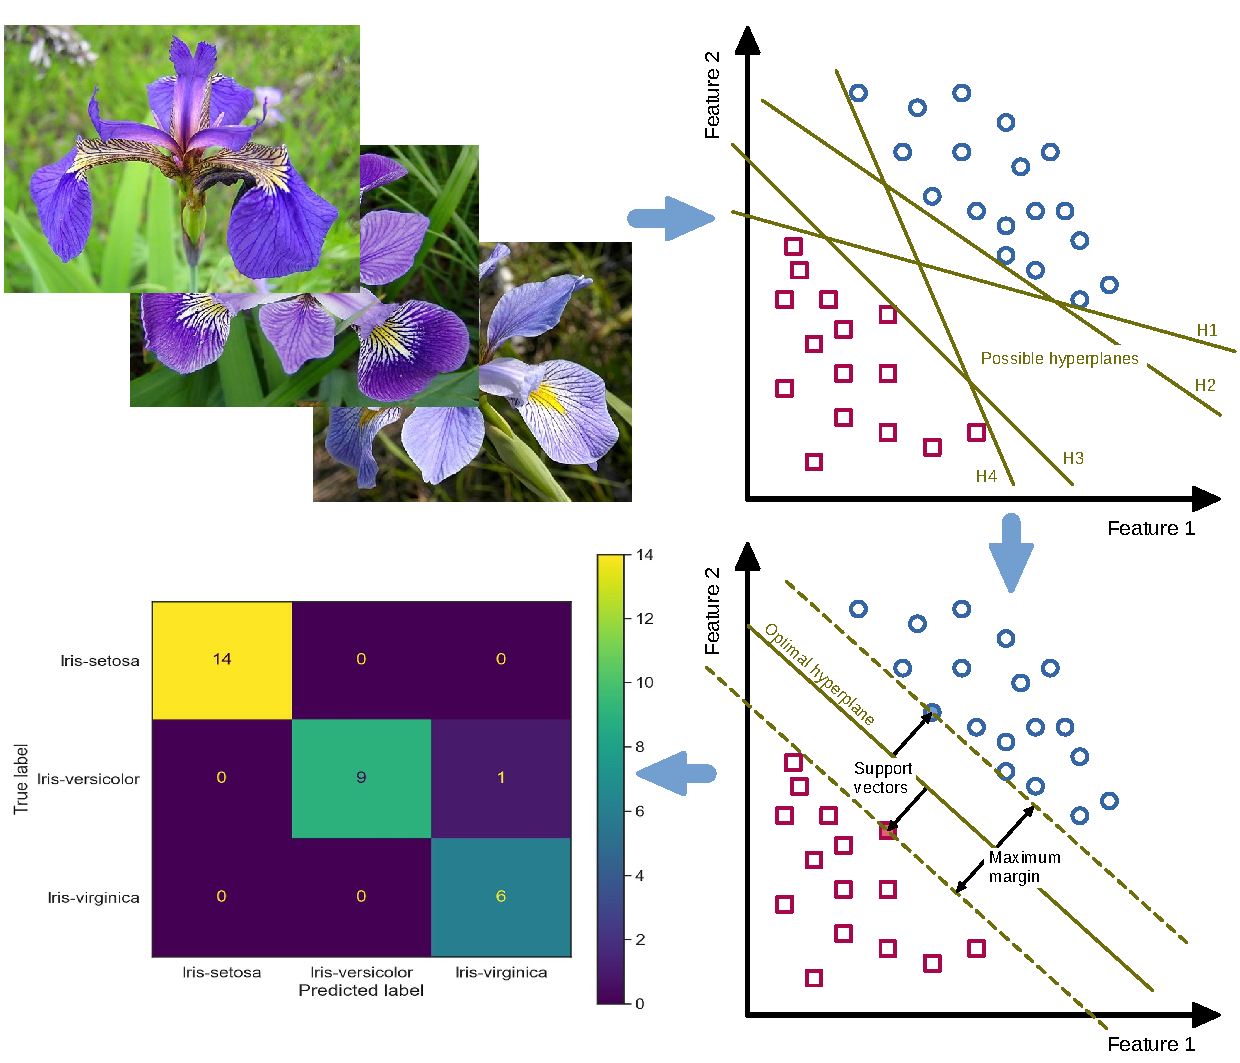
\includegraphics[width=0.90\textwidth]{images/Cover_image.pdf}
        \end{center}
        \vfill

    \begin{abstract}
    This is a placeholder for the abstract that needs to be added later.
    \end{abstract}
    \vfill
    
    \noindent
    \begin{center}
	    \begin{tabular}{>{\centering}m{0.2\textwidth}m{0.65\textwidth}}
	    \begin{minipage}{\linewidth}
	        
\includegraphics{images/CC_BY-SA_40.png}
	    \end{minipage}
	    &
	    \begin{minipage}{\linewidth}
	        This work is licensed under a \href{https://creativecommons.org/licenses/by-sa/4.0/}{Creative Commons Attribution-ShareAlike 4.0 International License (CC BY-SA 4.0)}.
	    \end{minipage}
	    \end{tabular}
	\end{center}

    \newpage

    % Activate own page style
    \pagestyle{fancy}
    % Delete all fields
    \fancyhf{}
    % \fancyhead[EL,OL]{$header$}
    % \fancyfoot[EL,OL]{$footer$}
    % Header leftside: chapter/section
    \fancyhead[ER,OR]{\leftmark}
    % Footer rightside: page number
    \fancyfoot[ER,OR]{Seite \thepage}

    \renewcommand{\sectionmark}[1]{
        \markboth{\thesection{} #1}{}
    }

    
    \tableofcontents
    
    


    
    \hypertarget{introduction}{%
\section{Introduction}\label{introduction}}

Why we use a
\href{https://en.wikipedia.org/wiki/Project_Jupyter}{Jupyter} notebook
to to publish the R program examples:

Jupyter is a new \textbf{open source} alternative to the proprietary
numerical software
\href{https://en.wikipedia.org/wiki/Wolfram_Mathematica}{Mathematica}
from \textbf{Wolfram Research} that is well on the way to become a
\textbf{standard for exchanging research results}
(\cite{Scientific_Paper_obsolete_2018};
\cite{Future_of_Research_Paper_2018}).

Originally Jupyter was intended as an IDE for the programming languages
\textbf{Julia} and \textbf{Python}. Besides that it is also possible to
install other interpreter kernels, such as the
\textbf{\href{https://irkernel.github.io/installation/}{IRkernel}} for
R. This can be interesting if the IDE \textbf{RStudio Desktop} is not
available on the target platform used. For example, it is very difficult
to install RStudio on the ARM-based embedded computer \textbf{Raspberry
Pi} due to many technical dependencies. In contrast, using the R kernel
in JupyterLab on the Raspberry Pi works very well and performant.

    \hypertarget{global-settings-and-dependencies}{%
\section{Global settings and
dependencies}\label{global-settings-and-dependencies}}

\hypertarget{install-missing-packages-if-not-present-yet}{%
\subsection{Install missing packages if not present
yet}\label{install-missing-packages-if-not-present-yet}}

    \begin{tcolorbox}[breakable, size=fbox, boxrule=1pt, pad at break*=1mm,colback=cellbackground, colframe=cellborder]
\prompt{In}{incolor}{3}{\boxspacing}
\begin{Verbatim}[commandchars=\\\{\}]
\PY{c+c1}{\PYZsh{} List of R packages that are used in this script}
\PY{n}{list.of.packages} \PY{o}{\PYZlt{}\PYZhy{}} \PY{n+nf}{c}\PY{p}{(}\PY{l+s}{\PYZdq{}}\PY{l+s}{data.table\PYZdq{}}\PY{p}{)}

\PY{c+c1}{\PYZsh{} Query the already installed packages and save the missing ones in a new list}
\PY{n}{missing.packages} \PY{o}{\PYZlt{}\PYZhy{}} \PY{n}{list.of.packages}\PY{p}{[}\PY{o}{!}\PY{p}{(}\PY{n}{list.of.packages} \PY{o}{\PYZpc{}in\PYZpc{}} \PY{n+nf}{installed.packages}\PY{p}{(}\PY{p}{)}\PY{p}{[}\PY{p}{,}\PY{l+s}{\PYZdq{}}\PY{l+s}{Package\PYZdq{}}\PY{p}{]}\PY{p}{)}\PY{p}{]}

\PY{c+c1}{\PYZsh{} Install missing packages}
\PY{n+nf}{if}\PY{p}{(}\PY{n+nf}{length}\PY{p}{(}\PY{n}{missing.packages}\PY{p}{)}\PY{p}{)} \PY{p}{\PYZob{}}
    \PY{n+nf}{install.packages}\PY{p}{(}\PY{n}{missing.packages}\PY{p}{)}
\PY{p}{\PYZcb{}} \PY{n}{else} \PY{p}{\PYZob{}}
    \PY{n+nf}{print}\PY{p}{(}\PY{l+s}{\PYZdq{}}\PY{l+s}{All required packages are installed.\PYZdq{}}\PY{p}{)}
\PY{p}{\PYZcb{}}
\end{Verbatim}
\end{tcolorbox}

    \begin{Verbatim}[commandchars=\\\{\}]
[1] "All required packages are installed."
    \end{Verbatim}

    \hypertarget{load-package-data.table}{%
\subsection{\texorpdfstring{Load package
\texttt{data.table}}{Load package data.table}}\label{load-package-data.table}}

The package \texttt{data.table} is used for reading and manipulating
tables (\texttt{data.table} inherits from \texttt{data.frame}). Install
and load it:

    \begin{tcolorbox}[breakable, size=fbox, boxrule=1pt, pad at break*=1mm,colback=cellbackground, colframe=cellborder]
\prompt{In}{incolor}{4}{\boxspacing}
\begin{Verbatim}[commandchars=\\\{\}]
\PY{n+nf}{library}\PY{p}{(}\PY{n}{data.table}\PY{p}{)}
\end{Verbatim}
\end{tcolorbox}

    \hypertarget{set-globally-used-input-and-output-folders}{%
\subsection{Set globally used input and output
folders}\label{set-globally-used-input-and-output-folders}}

    \begin{tcolorbox}[breakable, size=fbox, boxrule=1pt, pad at break*=1mm,colback=cellbackground, colframe=cellborder]
\prompt{In}{incolor}{5}{\boxspacing}
\begin{Verbatim}[commandchars=\\\{\}]
\PY{n}{str\PYZus{}input\PYZus{}path} \PY{o}{=} \PY{l+s}{\PYZdq{}}\PY{l+s}{./input\PYZus{}data\PYZus{}from\PYZus{}survey\PYZdq{}}
\PY{n}{str\PYZus{}output\PYZus{}path} \PY{o}{=} \PY{l+s}{\PYZdq{}}\PY{l+s}{./output\PYZus{}data\PYZus{}manipulated\PYZdq{}}
\end{Verbatim}
\end{tcolorbox}

    \hypertarget{create-data-frame-table-handling-the-file-names-of-input-csv-data-raw-data-from-survey}{%
\subsection{Create data frame (table) handling the file names of input
CSV data (raw data from
survey)}\label{create-data-frame-table-handling-the-file-names-of-input-csv-data-raw-data-from-survey}}

    \begin{tcolorbox}[breakable, size=fbox, boxrule=1pt, pad at break*=1mm,colback=cellbackground, colframe=cellborder]
\prompt{In}{incolor}{6}{\boxspacing}
\begin{Verbatim}[commandchars=\\\{\}]
\PY{n}{df\PYZus{}csvInputFiles} \PY{o}{\PYZlt{}\PYZhy{}} \PY{n+nf}{data.table}\PY{p}{(}
  \PY{n}{file\PYZus{}idx} \PY{o}{=} \PY{l+m}{1}\PY{o}{:}\PY{l+m}{4}\PY{p}{,}
  \PY{n}{keys} \PY{o}{=} \PY{n+nf}{c}\PY{p}{(}\PY{l+s}{\PYZdq{}}\PY{l+s}{all\PYZdq{}}\PY{p}{,} \PY{l+s}{\PYZdq{}}\PY{l+s}{CA\PYZdq{}}\PY{p}{,} \PY{l+s}{\PYZdq{}}\PY{l+s}{NGO\PYZdq{}}\PY{p}{,} \PY{l+s}{\PYZdq{}}\PY{l+s}{PE\PYZdq{}}\PY{p}{)}\PY{p}{,}
  \PY{n}{filenames} \PY{o}{=} \PY{n+nf}{c}\PY{p}{(}\PY{l+s}{\PYZdq{}}\PY{l+s}{rdata\PYZus{}all\PYZus{}AHP\PYZus{}edible\PYZus{}Cities\PYZus{}2022\PYZhy{}03\PYZhy{}18\PYZus{}09\PYZhy{}53.csv\PYZdq{}}\PY{p}{,}
                \PY{l+s}{\PYZdq{}}\PY{l+s}{rdata\PYZus{}CA\PYZus{}AHP\PYZus{}edible\PYZus{}Cities\PYZus{}2022\PYZhy{}03\PYZhy{}18\PYZus{}10\PYZhy{}28.csv\PYZdq{}}\PY{p}{,}
                \PY{l+s}{\PYZdq{}}\PY{l+s}{rdata\PYZus{}NGO\PYZus{}AHP\PYZus{}edible\PYZus{}Cities\PYZus{}2022\PYZhy{}03\PYZhy{}18\PYZus{}10\PYZhy{}40.csv\PYZdq{}}\PY{p}{,}
                \PY{l+s}{\PYZdq{}}\PY{l+s}{rdata\PYZus{}PE\PYZus{}AHP\PYZus{}edible\PYZus{}Cities\PYZus{}2022\PYZhy{}03\PYZhy{}18\PYZus{}10\PYZhy{}41.csv\PYZdq{}}\PY{p}{)}\PY{p}{,}
  \PY{n}{descriptions} \PY{o}{=} \PY{n+nf}{c}\PY{p}{(}\PY{l+s}{\PYZdq{}}\PY{l+s}{all target groups together\PYZdq{}}\PY{p}{,}
                   \PY{l+s}{\PYZdq{}}\PY{l+s}{City Administrations\PYZdq{}}\PY{p}{,}
                   \PY{l+s}{\PYZdq{}}\PY{l+s}{Non\PYZhy{}Governmental Organisations\PYZdq{}}\PY{p}{,}
                   \PY{l+s}{\PYZdq{}}\PY{l+s}{Practitioners and Experts\PYZdq{}}\PY{p}{)}
\PY{p}{)}

\PY{n+nf}{print}\PY{p}{(}\PY{n}{df\PYZus{}csvInputFiles}\PY{p}{)}
\end{Verbatim}
\end{tcolorbox}

    \begin{Verbatim}[commandchars=\\\{\}]
   file\_idx keys                                        filenames
1:        1  all rdata\_all\_AHP\_edible\_Cities\_2022-03-18\_09-53.csv
2:        2   CA  rdata\_CA\_AHP\_edible\_Cities\_2022-03-18\_10-28.csv
3:        3  NGO rdata\_NGO\_AHP\_edible\_Cities\_2022-03-18\_10-40.csv
4:        4   PE  rdata\_PE\_AHP\_edible\_Cities\_2022-03-18\_10-41.csv
                     descriptions
1:     all target groups together
2:           City Administrations
3: Non-Governmental Organisations
4:      Practitioners and Experts
    \end{Verbatim}

    \hypertarget{functions-to-prepare-the-survey-data-for-further-analysis}{%
\section{Functions to prepare the survey data for further
analysis}\label{functions-to-prepare-the-survey-data-for-further-analysis}}

The following functions are used to read the survey data from the CSV
files and prepare the data structure for further analysis with the R
package \texttt{ahpsurvey}.

\hypertarget{function-to-read-the-survey-data-from-csv-files-to-dataframe-objects}{%
\subsection{Function to read the survey data from CSV files to dataframe
objects}\label{function-to-read-the-survey-data-from-csv-files-to-dataframe-objects}}

Define a function for reading in a CSV file to 4 different dateframes by
selecting different columns.

    \begin{tcolorbox}[breakable, size=fbox, boxrule=1pt, pad at break*=1mm,colback=cellbackground, colframe=cellborder]
\prompt{In}{incolor}{5}{\boxspacing}
\begin{Verbatim}[commandchars=\\\{\}]
\PY{n}{func\PYZus{}readCSVdata\PYZus{}to\PYZus{}dataframes} \PY{o}{\PYZlt{}\PYZhy{}} \PY{n+nf}{function}\PY{p}{(}\PY{n}{str\PYZus{}CSVfilename}\PY{p}{)} \PY{p}{\PYZob{}}
  
  \PY{n}{df\PYZus{}mySurvey\PYZus{}1} \PY{o}{\PYZlt{}\PYZhy{}} \PY{n+nf}{fread}\PY{p}{(}
    \PY{n}{file} \PY{o}{=} \PY{n}{str\PYZus{}CSVfilename}\PY{p}{,} \PY{n}{encoding} \PY{o}{=} \PY{l+s}{\PYZdq{}}\PY{l+s}{UTF\PYZhy{}8\PYZdq{}}\PY{p}{,}
    \PY{n}{header} \PY{o}{=} \PY{k+kc}{TRUE}\PY{p}{,} \PY{n}{sep} \PY{o}{=} \PY{l+s}{\PYZdq{}}\PY{l+s}{\PYZbs{}t\PYZdq{}}\PY{p}{,} \PY{n}{quote} \PY{o}{=} \PY{l+s}{\PYZdq{}}\PY{l+s}{\PYZbs{}\PYZdq{}\PYZdq{}}\PY{p}{,}
    \PY{c+c1}{\PYZsh{} dec = \PYZdq{}.\PYZdq{}, row.names = \PYZdq{}CASE\PYZdq{},}
    \PY{n}{select} \PY{o}{=} \PY{n+nf}{c}\PY{p}{(}\PY{l+s}{\PYZdq{}}\PY{l+s}{CASE\PYZdq{}}\PY{p}{,} \PY{l+s}{\PYZdq{}}\PY{l+s}{AU01\PYZdq{}}\PY{p}{,} \PY{l+s}{\PYZdq{}}\PY{l+s}{AU02\PYZdq{}}\PY{p}{,} \PY{l+s}{\PYZdq{}}\PY{l+s}{AU03\PYZdq{}}\PY{p}{,} 
               \PY{l+s}{\PYZdq{}}\PY{l+s}{RU01\PYZus{}01\PYZdq{}}\PY{p}{,} \PY{l+s}{\PYZdq{}}\PY{l+s}{RU02\PYZus{}01\PYZdq{}}\PY{p}{,} \PY{l+s}{\PYZdq{}}\PY{l+s}{RU03\PYZus{}01\PYZdq{}}\PY{p}{,} \PY{l+s}{\PYZdq{}}\PY{l+s}{RU04\PYZus{}01\PYZdq{}}\PY{p}{,} \PY{l+s}{\PYZdq{}}\PY{l+s}{RU05\PYZus{}01\PYZdq{}}\PY{p}{,} \PY{l+s}{\PYZdq{}}\PY{l+s}{RU06\PYZus{}01\PYZdq{}}\PY{p}{)}
    \PY{p}{)}
  
  \PY{n}{df\PYZus{}mySurvey\PYZus{}2} \PY{o}{\PYZlt{}\PYZhy{}} \PY{n+nf}{fread}\PY{p}{(}
    \PY{n}{file} \PY{o}{=} \PY{n}{str\PYZus{}CSVfilename}\PY{p}{,} \PY{n}{encoding} \PY{o}{=} \PY{l+s}{\PYZdq{}}\PY{l+s}{UTF\PYZhy{}8\PYZdq{}}\PY{p}{,}
    \PY{n}{header} \PY{o}{=} \PY{k+kc}{TRUE}\PY{p}{,} \PY{n}{sep} \PY{o}{=} \PY{l+s}{\PYZdq{}}\PY{l+s}{\PYZbs{}t\PYZdq{}}\PY{p}{,} \PY{n}{quote} \PY{o}{=} \PY{l+s}{\PYZdq{}}\PY{l+s}{\PYZbs{}\PYZdq{}\PYZdq{}}\PY{p}{,}
    \PY{c+c1}{\PYZsh{} dec = \PYZdq{}.\PYZdq{}, row.names = \PYZdq{}CASE\PYZdq{},}
    \PY{n}{select} \PY{o}{=} \PY{n+nf}{c}\PY{p}{(}\PY{l+s}{\PYZdq{}}\PY{l+s}{CASE\PYZdq{}}\PY{p}{,} \PY{l+s}{\PYZdq{}}\PY{l+s}{AS01\PYZdq{}}\PY{p}{,} \PY{l+s}{\PYZdq{}}\PY{l+s}{AS02\PYZdq{}}\PY{p}{,} \PY{l+s}{\PYZdq{}}\PY{l+s}{AS03\PYZdq{}}\PY{p}{,} 
               \PY{l+s}{\PYZdq{}}\PY{l+s}{RS01\PYZus{}01\PYZdq{}}\PY{p}{,} \PY{l+s}{\PYZdq{}}\PY{l+s}{RS02\PYZus{}01\PYZdq{}}\PY{p}{,} \PY{l+s}{\PYZdq{}}\PY{l+s}{RS03\PYZus{}01\PYZdq{}}\PY{p}{,} \PY{l+s}{\PYZdq{}}\PY{l+s}{RS04\PYZus{}01\PYZdq{}}\PY{p}{,} \PY{l+s}{\PYZdq{}}\PY{l+s}{RS05\PYZus{}01\PYZdq{}}\PY{p}{,} \PY{l+s}{\PYZdq{}}\PY{l+s}{RS06\PYZus{}01\PYZdq{}}\PY{p}{)}
    \PY{p}{)}
  
  \PY{n}{df\PYZus{}mySurvey\PYZus{}3} \PY{o}{\PYZlt{}\PYZhy{}} \PY{n+nf}{fread}\PY{p}{(}
    \PY{n}{file} \PY{o}{=} \PY{n}{str\PYZus{}CSVfilename}\PY{p}{,} \PY{n}{encoding} \PY{o}{=} \PY{l+s}{\PYZdq{}}\PY{l+s}{UTF\PYZhy{}8\PYZdq{}}\PY{p}{,}
    \PY{n}{header} \PY{o}{=} \PY{k+kc}{TRUE}\PY{p}{,} \PY{n}{sep} \PY{o}{=} \PY{l+s}{\PYZdq{}}\PY{l+s}{\PYZbs{}t\PYZdq{}}\PY{p}{,} \PY{n}{quote} \PY{o}{=} \PY{l+s}{\PYZdq{}}\PY{l+s}{\PYZbs{}\PYZdq{}\PYZdq{}}\PY{p}{,}
    \PY{c+c1}{\PYZsh{} dec = \PYZdq{}.\PYZdq{}, row.names = \PYZdq{}CASE\PYZdq{},}
    \PY{n}{select} \PY{o}{=} \PY{n+nf}{c}\PY{p}{(}\PY{l+s}{\PYZdq{}}\PY{l+s}{CASE\PYZdq{}}\PY{p}{,} \PY{l+s}{\PYZdq{}}\PY{l+s}{AW01\PYZdq{}}\PY{p}{,} \PY{l+s}{\PYZdq{}}\PY{l+s}{AW02\PYZdq{}}\PY{p}{,} \PY{l+s}{\PYZdq{}}\PY{l+s}{AW03\PYZdq{}}\PY{p}{,} 
               \PY{l+s}{\PYZdq{}}\PY{l+s}{RW01\PYZus{}01\PYZdq{}}\PY{p}{,} \PY{l+s}{\PYZdq{}}\PY{l+s}{RW02\PYZus{}01\PYZdq{}}\PY{p}{,} \PY{l+s}{\PYZdq{}}\PY{l+s}{RW03\PYZus{}01\PYZdq{}}\PY{p}{,} \PY{l+s}{\PYZdq{}}\PY{l+s}{RW04\PYZus{}01\PYZdq{}}\PY{p}{,} \PY{l+s}{\PYZdq{}}\PY{l+s}{RW05\PYZus{}01\PYZdq{}}\PY{p}{,} \PY{l+s}{\PYZdq{}}\PY{l+s}{RW06\PYZus{}01\PYZdq{}}\PY{p}{)}
    \PY{p}{)}
  
  \PY{n}{df\PYZus{}mySurvey\PYZus{}4} \PY{o}{\PYZlt{}\PYZhy{}} \PY{n+nf}{fread}\PY{p}{(}
    \PY{n}{file} \PY{o}{=} \PY{n}{str\PYZus{}CSVfilename}\PY{p}{,} \PY{n}{encoding} \PY{o}{=} \PY{l+s}{\PYZdq{}}\PY{l+s}{UTF\PYZhy{}8\PYZdq{}}\PY{p}{,}
    \PY{n}{header} \PY{o}{=} \PY{k+kc}{TRUE}\PY{p}{,} \PY{n}{sep} \PY{o}{=} \PY{l+s}{\PYZdq{}}\PY{l+s}{\PYZbs{}t\PYZdq{}}\PY{p}{,} \PY{n}{quote} \PY{o}{=} \PY{l+s}{\PYZdq{}}\PY{l+s}{\PYZbs{}\PYZdq{}\PYZdq{}}\PY{p}{,}
    \PY{c+c1}{\PYZsh{} dec = \PYZdq{}.\PYZdq{}, row.var = \PYZdq{}CASE\PYZdq{},}
    \PY{n}{select} \PY{o}{=} \PY{n+nf}{c}\PY{p}{(}\PY{l+s}{\PYZdq{}}\PY{l+s}{CASE\PYZdq{}}\PY{p}{,} \PY{l+s}{\PYZdq{}}\PY{l+s}{AK01\PYZdq{}}\PY{p}{,} \PY{l+s}{\PYZdq{}}\PY{l+s}{AK02\PYZdq{}}\PY{p}{,} \PY{l+s}{\PYZdq{}}\PY{l+s}{AK03\PYZdq{}}\PY{p}{,} 
               \PY{l+s}{\PYZdq{}}\PY{l+s}{RK01\PYZus{}01\PYZdq{}}\PY{p}{,} \PY{l+s}{\PYZdq{}}\PY{l+s}{RK02\PYZus{}01\PYZdq{}}\PY{p}{,} \PY{l+s}{\PYZdq{}}\PY{l+s}{RK03\PYZus{}01\PYZdq{}}\PY{p}{,} \PY{l+s}{\PYZdq{}}\PY{l+s}{RK04\PYZus{}01\PYZdq{}}\PY{p}{,} \PY{l+s}{\PYZdq{}}\PY{l+s}{RK05\PYZus{}01\PYZdq{}}\PY{p}{,} \PY{l+s}{\PYZdq{}}\PY{l+s}{RK06\PYZus{}01\PYZdq{}}\PY{p}{)}
    \PY{p}{)}
  
  \PY{n}{output} \PY{o}{\PYZlt{}\PYZhy{}} \PY{n+nf}{list}\PY{p}{(}\PY{n}{df\PYZus{}mySurvey\PYZus{}1}\PY{p}{,} \PY{n}{df\PYZus{}mySurvey\PYZus{}2}\PY{p}{,} \PY{n}{df\PYZus{}mySurvey\PYZus{}3}\PY{p}{,} \PY{n}{df\PYZus{}mySurvey\PYZus{}4}\PY{p}{)}
  
  \PY{n+nf}{return}\PY{p}{(}\PY{n}{output}\PY{p}{)}
\PY{p}{\PYZcb{}}
\end{Verbatim}
\end{tcolorbox}

    \hypertarget{function-to-prepare-the-data-and-store-it-in-new-dataframes}{%
\subsection{Function to prepare the data and store it in new
dataframes}\label{function-to-prepare-the-data-and-store-it-in-new-dataframes}}

    \begin{tcolorbox}[breakable, size=fbox, boxrule=1pt, pad at break*=1mm,colback=cellbackground, colframe=cellborder]
\prompt{In}{incolor}{6}{\boxspacing}
\begin{Verbatim}[commandchars=\\\{\}]
\PY{n}{func\PYZus{}scrambleData} \PY{o}{\PYZlt{}\PYZhy{}} \PY{n+nf}{function}\PY{p}{(}\PY{n}{df\PYZus{}inputData}\PY{p}{,} \PY{n}{vec\PYZus{}colnames\PYZus{}search\PYZus{}1}\PY{p}{,} \PY{n}{vec\PYZus{}colnames\PYZus{}search\PYZus{}2}\PY{p}{,} \PY{n}{vec\PYZus{}colnames\PYZus{}out}\PY{p}{)} \PY{p}{\PYZob{}}
  \PY{c+c1}{\PYZsh{} Generate new data frame ...}
  \PY{n}{df\PYZus{}outputData} \PY{o}{\PYZlt{}\PYZhy{}} \PY{n+nf}{data.frame}\PY{p}{(}\PY{n+nf}{matrix}\PY{p}{(}\PY{n}{ncol} \PY{o}{=} \PY{l+m}{3}\PY{p}{,} \PY{n}{nrow} \PY{o}{=} \PY{l+m}{0}\PY{p}{)}\PY{p}{)}
  \PY{c+c1}{\PYZsh{} ... and name the columns}
  \PY{n+nf}{colnames}\PY{p}{(}\PY{n}{df\PYZus{}outputData}\PY{p}{)} \PY{o}{\PYZlt{}\PYZhy{}} \PY{n}{vec\PYZus{}colnames\PYZus{}out}
  
  \PY{c+c1}{\PYZsh{} Generate 1. column}
  \PY{n+nf}{for }\PY{p}{(} \PY{n}{row\PYZus{}idx} \PY{n}{in} \PY{l+m}{1}\PY{o}{:}\PY{n+nf}{nrow}\PY{p}{(}\PY{n}{df\PYZus{}inputData}\PY{p}{)} \PY{p}{)} \PY{p}{\PYZob{}}
    \PY{c+c1}{\PYZsh{} filter column names by vector element}
    \PY{n+nf}{if }\PY{p}{(}\PY{n}{df\PYZus{}inputData}\PY{p}{[}\PY{n}{row\PYZus{}idx}\PY{p}{,} \PY{n+nf}{colnames}\PY{p}{(}\PY{n}{df\PYZus{}inputData}\PY{p}{)} \PY{o}{\PYZpc{}in\PYZpc{}} \PY{n}{vec\PYZus{}colnames\PYZus{}search\PYZus{}1}\PY{p}{[}\PY{l+m}{1}\PY{p}{]}\PY{p}{,} \PY{n}{with}\PY{o}{=}\PY{k+kc}{FALSE}\PY{p}{]} \PY{o}{==} \PY{l+m}{1}\PY{p}{)} \PY{p}{\PYZob{}}
      \PY{n}{int\PYZus{}tmp\PYZus{}val} \PY{o}{\PYZlt{}\PYZhy{}} \PY{n+nf}{as.integer}\PY{p}{(}\PY{n}{df\PYZus{}inputData}\PY{p}{[}\PY{n}{row\PYZus{}idx}\PY{p}{,} \PY{n+nf}{colnames}\PY{p}{(}\PY{n}{df\PYZus{}inputData}\PY{p}{)} \PY{o}{\PYZpc{}in\PYZpc{}} \PY{n}{vec\PYZus{}colnames\PYZus{}search\PYZus{}2}\PY{p}{[}\PY{l+m}{1}\PY{p}{]}\PY{p}{,} \PY{n}{with}\PY{o}{=}\PY{k+kc}{FALSE}\PY{p}{]}\PY{p}{)}
      \PY{n}{int\PYZus{}tmp\PYZus{}val} \PY{o}{\PYZlt{}\PYZhy{}} \PY{n}{int\PYZus{}tmp\PYZus{}val} \PY{o}{*} \PY{l+m}{\PYZhy{}1} \PY{o}{\PYZhy{}} \PY{l+m}{1}

      \PY{n}{df\PYZus{}outputData}\PY{p}{[}\PY{n}{row\PYZus{}idx}\PY{p}{,} \PY{n}{vec\PYZus{}colnames\PYZus{}out}\PY{p}{[}\PY{l+m}{1}\PY{p}{]]} \PY{o}{\PYZlt{}\PYZhy{}} \PY{n}{int\PYZus{}tmp\PYZus{}val}
    \PY{p}{\PYZcb{}}
    \PY{n}{else} \PY{n+nf}{if }\PY{p}{(}\PY{n}{df\PYZus{}inputData}\PY{p}{[}\PY{n}{row\PYZus{}idx}\PY{p}{,} \PY{n+nf}{colnames}\PY{p}{(}\PY{n}{df\PYZus{}inputData}\PY{p}{)} \PY{o}{\PYZpc{}in\PYZpc{}} \PY{n}{vec\PYZus{}colnames\PYZus{}search\PYZus{}1}\PY{p}{[}\PY{l+m}{1}\PY{p}{]}\PY{p}{,} \PY{n}{with}\PY{o}{=}\PY{k+kc}{FALSE}\PY{p}{]} \PY{o}{==} \PY{l+m}{\PYZhy{}1}\PY{p}{)} \PY{p}{\PYZob{}}
      \PY{n}{df\PYZus{}outputData}\PY{p}{[}\PY{n}{row\PYZus{}idx}\PY{p}{,} \PY{n}{vec\PYZus{}colnames\PYZus{}out}\PY{p}{[}\PY{l+m}{1}\PY{p}{]]} \PY{o}{\PYZlt{}\PYZhy{}} \PY{l+m}{1}
    \PY{p}{\PYZcb{}}
    \PY{n}{else} \PY{n+nf}{if }\PY{p}{(}\PY{n}{df\PYZus{}inputData}\PY{p}{[}\PY{n}{row\PYZus{}idx}\PY{p}{,} \PY{n+nf}{colnames}\PY{p}{(}\PY{n}{df\PYZus{}inputData}\PY{p}{)} \PY{o}{\PYZpc{}in\PYZpc{}} \PY{n}{vec\PYZus{}colnames\PYZus{}search\PYZus{}1}\PY{p}{[}\PY{l+m}{1}\PY{p}{]}\PY{p}{,} \PY{n}{with}\PY{o}{=}\PY{k+kc}{FALSE}\PY{p}{]} \PY{o}{==} \PY{l+m}{2}\PY{p}{)} \PY{p}{\PYZob{}}
      \PY{n}{int\PYZus{}tmp\PYZus{}val} \PY{o}{\PYZlt{}\PYZhy{}} \PY{n+nf}{as.integer}\PY{p}{(}\PY{n}{df\PYZus{}inputData}\PY{p}{[}\PY{n}{row\PYZus{}idx}\PY{p}{,} \PY{n+nf}{colnames}\PY{p}{(}\PY{n}{df\PYZus{}inputData}\PY{p}{)} \PY{o}{\PYZpc{}in\PYZpc{}} \PY{n}{vec\PYZus{}colnames\PYZus{}search\PYZus{}2}\PY{p}{[}\PY{l+m}{2}\PY{p}{]}\PY{p}{,} \PY{n}{with}\PY{o}{=}\PY{k+kc}{FALSE}\PY{p}{]}\PY{p}{)}
      \PY{n}{int\PYZus{}tmp\PYZus{}val} \PY{o}{\PYZlt{}\PYZhy{}} \PY{n}{int\PYZus{}tmp\PYZus{}val} \PY{o}{+} \PY{l+m}{1}

      \PY{n}{df\PYZus{}outputData}\PY{p}{[}\PY{n}{row\PYZus{}idx}\PY{p}{,} \PY{n}{vec\PYZus{}colnames\PYZus{}out}\PY{p}{[}\PY{l+m}{1}\PY{p}{]]} \PY{o}{\PYZlt{}\PYZhy{}} \PY{n}{int\PYZus{}tmp\PYZus{}val}
    \PY{p}{\PYZcb{}}
  \PY{p}{\PYZcb{}}
  
  \PY{c+c1}{\PYZsh{} Generate 2. column}
  \PY{n+nf}{for }\PY{p}{(} \PY{n}{row\PYZus{}idx} \PY{n}{in} \PY{l+m}{1}\PY{o}{:}\PY{n+nf}{nrow}\PY{p}{(}\PY{n}{df\PYZus{}inputData}\PY{p}{)} \PY{p}{)} \PY{p}{\PYZob{}}
    \PY{c+c1}{\PYZsh{} filter column names by vector element}
    \PY{n+nf}{if }\PY{p}{(}\PY{n}{df\PYZus{}inputData}\PY{p}{[}\PY{n}{row\PYZus{}idx}\PY{p}{,} \PY{n+nf}{colnames}\PY{p}{(}\PY{n}{df\PYZus{}inputData}\PY{p}{)} \PY{o}{\PYZpc{}in\PYZpc{}} \PY{n}{vec\PYZus{}colnames\PYZus{}search\PYZus{}1}\PY{p}{[}\PY{l+m}{2}\PY{p}{]}\PY{p}{,} \PY{n}{with}\PY{o}{=}\PY{k+kc}{FALSE}\PY{p}{]} \PY{o}{==} \PY{l+m}{1}\PY{p}{)} \PY{p}{\PYZob{}}
      \PY{n}{int\PYZus{}tmp\PYZus{}val} \PY{o}{\PYZlt{}\PYZhy{}} \PY{n+nf}{as.integer}\PY{p}{(}\PY{n}{df\PYZus{}inputData}\PY{p}{[}\PY{n}{row\PYZus{}idx}\PY{p}{,} \PY{n+nf}{colnames}\PY{p}{(}\PY{n}{df\PYZus{}inputData}\PY{p}{)} \PY{o}{\PYZpc{}in\PYZpc{}} \PY{n}{vec\PYZus{}colnames\PYZus{}search\PYZus{}2}\PY{p}{[}\PY{l+m}{3}\PY{p}{]}\PY{p}{,} \PY{n}{with}\PY{o}{=}\PY{k+kc}{FALSE}\PY{p}{]}\PY{p}{)}
      \PY{n}{int\PYZus{}tmp\PYZus{}val} \PY{o}{\PYZlt{}\PYZhy{}} \PY{n}{int\PYZus{}tmp\PYZus{}val} \PY{o}{*} \PY{l+m}{\PYZhy{}1} \PY{o}{\PYZhy{}} \PY{l+m}{1}
      
      \PY{n}{df\PYZus{}outputData}\PY{p}{[}\PY{n}{row\PYZus{}idx}\PY{p}{,} \PY{n}{vec\PYZus{}colnames\PYZus{}out}\PY{p}{[}\PY{l+m}{2}\PY{p}{]]} \PY{o}{\PYZlt{}\PYZhy{}} \PY{n}{int\PYZus{}tmp\PYZus{}val}
    \PY{p}{\PYZcb{}} 
    \PY{n}{else} \PY{n+nf}{if }\PY{p}{(}\PY{n}{df\PYZus{}inputData}\PY{p}{[}\PY{n}{row\PYZus{}idx}\PY{p}{,} \PY{n+nf}{colnames}\PY{p}{(}\PY{n}{df\PYZus{}inputData}\PY{p}{)} \PY{o}{\PYZpc{}in\PYZpc{}} \PY{n}{vec\PYZus{}colnames\PYZus{}search\PYZus{}1}\PY{p}{[}\PY{l+m}{2}\PY{p}{]}\PY{p}{,} \PY{n}{with}\PY{o}{=}\PY{k+kc}{FALSE}\PY{p}{]} \PY{o}{==} \PY{l+m}{\PYZhy{}1}\PY{p}{)} \PY{p}{\PYZob{}}
      \PY{n}{df\PYZus{}outputData}\PY{p}{[}\PY{n}{row\PYZus{}idx}\PY{p}{,} \PY{n}{vec\PYZus{}colnames\PYZus{}out}\PY{p}{[}\PY{l+m}{2}\PY{p}{]]} \PY{o}{\PYZlt{}\PYZhy{}} \PY{l+m}{1}
    \PY{p}{\PYZcb{}} 
    \PY{n}{else} \PY{n+nf}{if }\PY{p}{(}\PY{n}{df\PYZus{}inputData}\PY{p}{[}\PY{n}{row\PYZus{}idx}\PY{p}{,} \PY{n+nf}{colnames}\PY{p}{(}\PY{n}{df\PYZus{}inputData}\PY{p}{)} \PY{o}{\PYZpc{}in\PYZpc{}} \PY{n}{vec\PYZus{}colnames\PYZus{}search\PYZus{}1}\PY{p}{[}\PY{l+m}{2}\PY{p}{]}\PY{p}{,} \PY{n}{with}\PY{o}{=}\PY{k+kc}{FALSE}\PY{p}{]} \PY{o}{==} \PY{l+m}{2}\PY{p}{)} \PY{p}{\PYZob{}}
      \PY{n}{int\PYZus{}tmp\PYZus{}val} \PY{o}{\PYZlt{}\PYZhy{}} \PY{n+nf}{as.integer}\PY{p}{(}\PY{n}{df\PYZus{}inputData}\PY{p}{[}\PY{n}{row\PYZus{}idx}\PY{p}{,} \PY{n+nf}{colnames}\PY{p}{(}\PY{n}{df\PYZus{}inputData}\PY{p}{)} \PY{o}{\PYZpc{}in\PYZpc{}} \PY{n}{vec\PYZus{}colnames\PYZus{}search\PYZus{}2}\PY{p}{[}\PY{l+m}{4}\PY{p}{]}\PY{p}{,} \PY{n}{with}\PY{o}{=}\PY{k+kc}{FALSE}\PY{p}{]}\PY{p}{)}
      \PY{n}{int\PYZus{}tmp\PYZus{}val} \PY{o}{\PYZlt{}\PYZhy{}} \PY{n}{int\PYZus{}tmp\PYZus{}val} \PY{o}{+} \PY{l+m}{1}
      
      \PY{n}{df\PYZus{}outputData}\PY{p}{[}\PY{n}{row\PYZus{}idx}\PY{p}{,} \PY{n}{vec\PYZus{}colnames\PYZus{}out}\PY{p}{[}\PY{l+m}{2}\PY{p}{]]} \PY{o}{\PYZlt{}\PYZhy{}} \PY{n}{int\PYZus{}tmp\PYZus{}val}
    \PY{p}{\PYZcb{}}
  \PY{p}{\PYZcb{}}
  
  \PY{c+c1}{\PYZsh{} Generate 3. column}
  \PY{n+nf}{for }\PY{p}{(} \PY{n}{row\PYZus{}idx} \PY{n}{in} \PY{l+m}{1}\PY{o}{:}\PY{n+nf}{nrow}\PY{p}{(}\PY{n}{df\PYZus{}inputData}\PY{p}{)} \PY{p}{)} \PY{p}{\PYZob{}}
    \PY{c+c1}{\PYZsh{} filter column names by vector element}
    \PY{n+nf}{if }\PY{p}{(}\PY{n}{df\PYZus{}inputData}\PY{p}{[}\PY{n}{row\PYZus{}idx}\PY{p}{,} \PY{n+nf}{colnames}\PY{p}{(}\PY{n}{df\PYZus{}inputData}\PY{p}{)} \PY{o}{\PYZpc{}in\PYZpc{}} \PY{n}{vec\PYZus{}colnames\PYZus{}search\PYZus{}1}\PY{p}{[}\PY{l+m}{3}\PY{p}{]}\PY{p}{,} \PY{n}{with}\PY{o}{=}\PY{k+kc}{FALSE}\PY{p}{]} \PY{o}{==} \PY{l+m}{1}\PY{p}{)} \PY{p}{\PYZob{}}
      \PY{n}{int\PYZus{}tmp\PYZus{}val} \PY{o}{\PYZlt{}\PYZhy{}} \PY{n+nf}{as.integer}\PY{p}{(}\PY{n}{df\PYZus{}inputData}\PY{p}{[}\PY{n}{row\PYZus{}idx}\PY{p}{,} \PY{n+nf}{colnames}\PY{p}{(}\PY{n}{df\PYZus{}inputData}\PY{p}{)} \PY{o}{\PYZpc{}in\PYZpc{}} \PY{n}{vec\PYZus{}colnames\PYZus{}search\PYZus{}2}\PY{p}{[}\PY{l+m}{5}\PY{p}{]}\PY{p}{,} \PY{n}{with}\PY{o}{=}\PY{k+kc}{FALSE}\PY{p}{]}\PY{p}{)}
      \PY{n}{int\PYZus{}tmp\PYZus{}val} \PY{o}{\PYZlt{}\PYZhy{}} \PY{n}{int\PYZus{}tmp\PYZus{}val} \PY{o}{*} \PY{l+m}{\PYZhy{}1} \PY{o}{\PYZhy{}} \PY{l+m}{1}
      
      \PY{n}{df\PYZus{}outputData}\PY{p}{[}\PY{n}{row\PYZus{}idx}\PY{p}{,} \PY{n}{vec\PYZus{}colnames\PYZus{}out}\PY{p}{[}\PY{l+m}{3}\PY{p}{]]} \PY{o}{\PYZlt{}\PYZhy{}} \PY{n}{int\PYZus{}tmp\PYZus{}val}
    \PY{p}{\PYZcb{}} 
    \PY{n}{else} \PY{n+nf}{if }\PY{p}{(}\PY{n}{df\PYZus{}inputData}\PY{p}{[}\PY{n}{row\PYZus{}idx}\PY{p}{,} \PY{n+nf}{colnames}\PY{p}{(}\PY{n}{df\PYZus{}inputData}\PY{p}{)} \PY{o}{\PYZpc{}in\PYZpc{}} \PY{n}{vec\PYZus{}colnames\PYZus{}search\PYZus{}1}\PY{p}{[}\PY{l+m}{3}\PY{p}{]}\PY{p}{,} \PY{n}{with}\PY{o}{=}\PY{k+kc}{FALSE}\PY{p}{]} \PY{o}{==} \PY{l+m}{\PYZhy{}1}\PY{p}{)} \PY{p}{\PYZob{}}
      \PY{n}{df\PYZus{}outputData}\PY{p}{[}\PY{n}{row\PYZus{}idx}\PY{p}{,} \PY{n}{vec\PYZus{}colnames\PYZus{}out}\PY{p}{[}\PY{l+m}{3}\PY{p}{]]} \PY{o}{\PYZlt{}\PYZhy{}} \PY{l+m}{1}
    \PY{p}{\PYZcb{}} 
    \PY{n}{else} \PY{n+nf}{if }\PY{p}{(}\PY{n}{df\PYZus{}inputData}\PY{p}{[}\PY{n}{row\PYZus{}idx}\PY{p}{,} \PY{n+nf}{colnames}\PY{p}{(}\PY{n}{df\PYZus{}inputData}\PY{p}{)} \PY{o}{\PYZpc{}in\PYZpc{}} \PY{n}{vec\PYZus{}colnames\PYZus{}search\PYZus{}1}\PY{p}{[}\PY{l+m}{3}\PY{p}{]}\PY{p}{,} \PY{n}{with}\PY{o}{=}\PY{k+kc}{FALSE}\PY{p}{]} \PY{o}{==} \PY{l+m}{2}\PY{p}{)} \PY{p}{\PYZob{}}
      \PY{n}{int\PYZus{}tmp\PYZus{}val} \PY{o}{\PYZlt{}\PYZhy{}} \PY{n+nf}{as.integer}\PY{p}{(}\PY{n}{df\PYZus{}inputData}\PY{p}{[}\PY{n}{row\PYZus{}idx}\PY{p}{,} \PY{n+nf}{colnames}\PY{p}{(}\PY{n}{df\PYZus{}inputData}\PY{p}{)} \PY{o}{\PYZpc{}in\PYZpc{}} \PY{n}{vec\PYZus{}colnames\PYZus{}search\PYZus{}2}\PY{p}{[}\PY{l+m}{6}\PY{p}{]}\PY{p}{,} \PY{n}{with}\PY{o}{=}\PY{k+kc}{FALSE}\PY{p}{]}\PY{p}{)}
      \PY{n}{int\PYZus{}tmp\PYZus{}val} \PY{o}{\PYZlt{}\PYZhy{}} \PY{n}{int\PYZus{}tmp\PYZus{}val} \PY{o}{+} \PY{l+m}{1}
      
      \PY{n}{df\PYZus{}outputData}\PY{p}{[}\PY{n}{row\PYZus{}idx}\PY{p}{,} \PY{n}{vec\PYZus{}colnames\PYZus{}out}\PY{p}{[}\PY{l+m}{3}\PY{p}{]]} \PY{o}{\PYZlt{}\PYZhy{}} \PY{n}{int\PYZus{}tmp\PYZus{}val}
    \PY{p}{\PYZcb{}}
  \PY{p}{\PYZcb{}}
  
  \PY{c+c1}{\PYZsh{} return scrambled data frame}
  \PY{n+nf}{return}\PY{p}{(}\PY{n}{df\PYZus{}outputData}\PY{p}{)}
\PY{p}{\PYZcb{}}
\end{Verbatim}
\end{tcolorbox}

    \hypertarget{function-to-write-resulting-dataframes-to-csv-files}{%
\subsection{Function to write resulting dataframes to CSV
files}\label{function-to-write-resulting-dataframes-to-csv-files}}

    \begin{tcolorbox}[breakable, size=fbox, boxrule=1pt, pad at break*=1mm,colback=cellbackground, colframe=cellborder]
\prompt{In}{incolor}{7}{\boxspacing}
\begin{Verbatim}[commandchars=\\\{\}]
\PY{n}{func\PYZus{}writeDataframe\PYZus{}to\PYZus{}CSVfile} \PY{o}{\PYZlt{}\PYZhy{}} \PY{n+nf}{function}\PY{p}{(}\PY{n}{str\PYZus{}path}\PY{p}{,} \PY{n}{str\PYZus{}CSVfilename}\PY{p}{,} \PY{n}{df\PYZus{}dataframe}\PY{p}{,} \PY{n}{str\PYZus{}filenameExtension}\PY{p}{)} \PY{p}{\PYZob{}}
  \PY{c+c1}{\PYZsh{} Split file name on second underscore, found here: }
  \PY{c+c1}{\PYZsh{} https://stackoverflow.com/questions/32398427/r\PYZhy{}split\PYZhy{}a\PYZhy{}character\PYZhy{}string\PYZhy{}on\PYZhy{}the\PYZhy{}second\PYZhy{}underscore/32398489\PYZsh{}32398489}
  \PY{n}{list\PYZus{}str\PYZus{}split} \PY{o}{\PYZlt{}\PYZhy{}} \PY{n+nf}{strsplit}\PY{p}{(}\PY{n+nf}{sub}\PY{p}{(}\PY{l+s}{\PYZsq{}}\PY{l+s}{(\PYZca{}[\PYZca{}\PYZus{}]+\PYZus{}[\PYZca{}\PYZus{}]+)\PYZus{}(.*)\PYZdl{}\PYZsq{}}\PY{p}{,} \PY{l+s}{\PYZsq{}}\PY{l+s}{\PYZbs{}\PYZbs{}1 \PYZbs{}\PYZbs{}2\PYZsq{}}\PY{p}{,} \PY{n}{str\PYZus{}CSVfilename}\PY{p}{)}\PY{p}{,} \PY{l+s}{\PYZsq{}}\PY{l+s}{ \PYZsq{}}\PY{p}{)}
  
  \PY{c+c1}{\PYZsh{} extend the file name prefix and glue together with old suffix}
  \PY{n}{str\PYZus{}CSVfilename\PYZus{}extended} \PY{o}{\PYZlt{}\PYZhy{}} \PY{n+nf}{paste}\PY{p}{(}\PY{n}{list\PYZus{}str\PYZus{}split}\PY{p}{[[}\PY{l+m}{1}\PY{p}{]]}\PY{p}{[}\PY{l+m}{1}\PY{p}{]}\PY{p}{,} \PY{n}{str\PYZus{}filenameExtension}\PY{p}{,} \PY{n}{list\PYZus{}str\PYZus{}split}\PY{p}{[[}\PY{l+m}{1}\PY{p}{]]}\PY{p}{[}\PY{l+m}{2}\PY{p}{]}\PY{p}{,} \PY{n}{sep}\PY{o}{=}\PY{l+s}{\PYZdq{}}\PY{l+s}{\PYZus{}\PYZdq{}}\PY{p}{)}
  
  \PY{c+c1}{\PYZsh{} extend file name by path}
  \PY{n}{str\PYZus{}CSVfilename\PYZus{}extended} \PY{o}{\PYZlt{}\PYZhy{}} \PY{n+nf}{paste}\PY{p}{(}\PY{n}{str\PYZus{}path}\PY{p}{,} \PY{n}{str\PYZus{}CSVfilename\PYZus{}extended}\PY{p}{,} \PY{n}{sep}\PY{o}{=}\PY{l+s}{\PYZdq{}}\PY{l+s}{/\PYZdq{}}\PY{p}{)}
  
  \PY{n+nf}{write.table}\PY{p}{(}\PY{n}{df\PYZus{}dataframe}\PY{p}{,} \PY{n}{file} \PY{o}{=} \PY{n}{str\PYZus{}CSVfilename\PYZus{}extended}\PY{p}{,}
              \PY{n}{fileEncoding} \PY{o}{=} \PY{l+s}{\PYZdq{}}\PY{l+s}{UTF\PYZhy{}8\PYZdq{}}\PY{p}{,} \PY{n}{row.names} \PY{o}{=} \PY{k+kc}{FALSE}\PY{p}{,}
              \PY{n}{col.names} \PY{o}{=} \PY{k+kc}{TRUE}\PY{p}{,} \PY{n}{sep} \PY{o}{=} \PY{l+s}{\PYZdq{}}\PY{l+s}{\PYZbs{}t\PYZdq{}}\PY{p}{,} \PY{n}{quote} \PY{o}{=} \PY{k+kc}{TRUE}\PY{p}{)}
\PY{p}{\PYZcb{}}
\end{Verbatim}
\end{tcolorbox}

    \hypertarget{prepare-the-data-and-store-it-in-new-csv-files-for-each-criterion}{%
\section{Prepare the data and store it in new CSV files for each
criterion}\label{prepare-the-data-and-store-it-in-new-csv-files-for-each-criterion}}

\hypertarget{environmental-sub-criteria}{%
\subsection{Environmental
sub-criteria}\label{environmental-sub-criteria}}

Walk over all input CSV files, select necessary columns, filter cells by
given algorithm, and write the results to output CSV files:

    \begin{tcolorbox}[breakable, size=fbox, boxrule=1pt, pad at break*=1mm,colback=cellbackground, colframe=cellborder]
\prompt{In}{incolor}{8}{\boxspacing}
\begin{Verbatim}[commandchars=\\\{\}]
\PY{n}{vec\PYZus{}colnames\PYZus{}search\PYZus{}1} \PY{o}{\PYZlt{}\PYZhy{}} \PY{n+nf}{c}\PY{p}{(}\PY{l+s}{\PYZsq{}}\PY{l+s}{AU01\PYZsq{}}\PY{p}{,} \PY{l+s}{\PYZsq{}}\PY{l+s}{AU02\PYZsq{}}\PY{p}{,} \PY{l+s}{\PYZsq{}}\PY{l+s}{AU03\PYZsq{}}\PY{p}{)}
\PY{n}{vec\PYZus{}colnames\PYZus{}search\PYZus{}2} \PY{o}{\PYZlt{}\PYZhy{}} \PY{n+nf}{c}\PY{p}{(}\PY{l+s}{\PYZsq{}}\PY{l+s}{RU01\PYZus{}01\PYZsq{}}\PY{p}{,} \PY{l+s}{\PYZsq{}}\PY{l+s}{RU02\PYZus{}01\PYZsq{}}\PY{p}{,} \PY{l+s}{\PYZsq{}}\PY{l+s}{RU03\PYZus{}01\PYZsq{}}\PY{p}{,} \PY{l+s}{\PYZsq{}}\PY{l+s}{RU04\PYZus{}01\PYZsq{}}\PY{p}{,} \PY{l+s}{\PYZsq{}}\PY{l+s}{RU05\PYZus{}01\PYZsq{}}\PY{p}{,} \PY{l+s}{\PYZsq{}}\PY{l+s}{RU06\PYZus{}01\PYZsq{}}\PY{p}{)}
\PY{n}{vec\PYZus{}colnames\PYZus{}out} \PY{o}{\PYZlt{}\PYZhy{}} \PY{n+nf}{c}\PY{p}{(}\PY{l+s}{\PYZsq{}}\PY{l+s}{Clim\PYZus{}BDiv\PYZsq{}}\PY{p}{,} \PY{l+s}{\PYZsq{}}\PY{l+s}{Clim\PYZus{}CiEc\PYZsq{}}\PY{p}{,} \PY{l+s}{\PYZsq{}}\PY{l+s}{BDiv\PYZus{}CiEc\PYZsq{}}\PY{p}{)}

\PY{n+nf}{for }\PY{p}{(} \PY{n}{row\PYZus{}idx} \PY{n}{in} \PY{l+m}{1}\PY{o}{:}\PY{n+nf}{nrow}\PY{p}{(}\PY{n}{df\PYZus{}csvInputFiles}\PY{p}{)} \PY{p}{)} \PY{p}{\PYZob{}}
  \PY{c+c1}{\PYZsh{} create list of data frames from current input CSV file}
  \PY{n}{str\PYZus{}filename} \PY{o}{\PYZlt{}\PYZhy{}} \PY{n+nf}{paste}\PY{p}{(}\PY{n}{str\PYZus{}input\PYZus{}path}\PY{p}{,} \PY{n}{df\PYZus{}csvInputFiles}\PY{p}{[}\PY{n}{row\PYZus{}idx}\PY{p}{,} \PY{n}{filenames}\PY{p}{]}\PY{p}{,} \PY{n}{sep}\PY{o}{=}\PY{l+s}{\PYZdq{}}\PY{l+s}{/\PYZdq{}}\PY{p}{)}
  \PY{n}{list\PYZus{}dataframes} \PY{o}{\PYZlt{}\PYZhy{}} \PY{n+nf}{func\PYZus{}readCSVdata\PYZus{}to\PYZus{}dataframes}\PY{p}{(}\PY{n}{str\PYZus{}filename}\PY{p}{)}
  
  \PY{c+c1}{\PYZsh{} scramble the data frames}
  \PY{n}{df\PYZus{}scrambledData} \PY{o}{\PYZlt{}\PYZhy{}} \PY{n+nf}{func\PYZus{}scrambleData}\PY{p}{(}\PY{n}{list\PYZus{}dataframes}\PY{p}{[[}\PY{l+m}{1}\PY{p}{]]}\PY{p}{,} \PY{n}{vec\PYZus{}colnames\PYZus{}search\PYZus{}1}\PY{p}{,} \PY{n}{vec\PYZus{}colnames\PYZus{}search\PYZus{}2}\PY{p}{,} \PY{n}{vec\PYZus{}colnames\PYZus{}out}\PY{p}{)}
  
  \PY{c+c1}{\PYZsh{} write scrambled data frames to output CSV file}
  \PY{n+nf}{func\PYZus{}writeDataframe\PYZus{}to\PYZus{}CSVfile}\PY{p}{(}\PY{n}{str\PYZus{}output\PYZus{}path}\PY{p}{,} \PY{n}{df\PYZus{}csvInputFiles}\PY{p}{[}\PY{n}{row\PYZus{}idx}\PY{p}{,} \PY{n}{filenames}\PY{p}{]}\PY{p}{,} \PY{n}{df\PYZus{}scrambledData}\PY{p}{,} \PY{l+s}{\PYZdq{}}\PY{l+s}{env\PYZdq{}}\PY{p}{)}
\PY{p}{\PYZcb{}}
\end{Verbatim}
\end{tcolorbox}

    \hypertarget{social-sub-criteria}{%
\subsection{Social sub-criteria}\label{social-sub-criteria}}

Walk over all input CSV files, select necessary columns, filter cells by
given algorithm, and write the results to output CSV files:

    \begin{tcolorbox}[breakable, size=fbox, boxrule=1pt, pad at break*=1mm,colback=cellbackground, colframe=cellborder]
\prompt{In}{incolor}{9}{\boxspacing}
\begin{Verbatim}[commandchars=\\\{\}]
\PY{n}{vec\PYZus{}colnames\PYZus{}search\PYZus{}1} \PY{o}{\PYZlt{}\PYZhy{}} \PY{n+nf}{c}\PY{p}{(}\PY{l+s}{\PYZsq{}}\PY{l+s}{AS01\PYZsq{}}\PY{p}{,} \PY{l+s}{\PYZsq{}}\PY{l+s}{AS02\PYZsq{}}\PY{p}{,} \PY{l+s}{\PYZsq{}}\PY{l+s}{AS03\PYZsq{}}\PY{p}{)}
\PY{n}{vec\PYZus{}colnames\PYZus{}search\PYZus{}2} \PY{o}{\PYZlt{}\PYZhy{}} \PY{n+nf}{c}\PY{p}{(}\PY{l+s}{\PYZsq{}}\PY{l+s}{RS01\PYZus{}01\PYZsq{}}\PY{p}{,} \PY{l+s}{\PYZsq{}}\PY{l+s}{RS02\PYZus{}01\PYZsq{}}\PY{p}{,} \PY{l+s}{\PYZsq{}}\PY{l+s}{RS03\PYZus{}01\PYZsq{}}\PY{p}{,} \PY{l+s}{\PYZsq{}}\PY{l+s}{RS04\PYZus{}01\PYZsq{}}\PY{p}{,} \PY{l+s}{\PYZsq{}}\PY{l+s}{RS05\PYZus{}01\PYZsq{}}\PY{p}{,} \PY{l+s}{\PYZsq{}}\PY{l+s}{RS06\PYZus{}01\PYZsq{}}\PY{p}{)}
\PY{n}{vec\PYZus{}colnames\PYZus{}out} \PY{o}{\PYZlt{}\PYZhy{}} \PY{n+nf}{c}\PY{p}{(}\PY{l+s}{\PYZsq{}}\PY{l+s}{KEdu\PYZus{}Comm\PYZsq{}}\PY{p}{,} \PY{l+s}{\PYZsq{}}\PY{l+s}{KEdu\PYZus{}Part\PYZsq{}}\PY{p}{,} \PY{l+s}{\PYZsq{}}\PY{l+s}{Comm\PYZus{}Part\PYZsq{}}\PY{p}{)}

\PY{n+nf}{for }\PY{p}{(} \PY{n}{row\PYZus{}idx} \PY{n}{in} \PY{l+m}{1}\PY{o}{:}\PY{n+nf}{nrow}\PY{p}{(}\PY{n}{df\PYZus{}csvInputFiles}\PY{p}{)} \PY{p}{)} \PY{p}{\PYZob{}}
  \PY{c+c1}{\PYZsh{} create list of data frames from current input CSV file}
  \PY{n}{str\PYZus{}filename} \PY{o}{\PYZlt{}\PYZhy{}} \PY{n+nf}{paste}\PY{p}{(}\PY{n}{str\PYZus{}input\PYZus{}path}\PY{p}{,} \PY{n}{df\PYZus{}csvInputFiles}\PY{p}{[}\PY{n}{row\PYZus{}idx}\PY{p}{,} \PY{n}{filenames}\PY{p}{]}\PY{p}{,} \PY{n}{sep}\PY{o}{=}\PY{l+s}{\PYZdq{}}\PY{l+s}{/\PYZdq{}}\PY{p}{)}
  \PY{n}{list\PYZus{}dataframes} \PY{o}{\PYZlt{}\PYZhy{}} \PY{n+nf}{func\PYZus{}readCSVdata\PYZus{}to\PYZus{}dataframes}\PY{p}{(}\PY{n}{str\PYZus{}filename}\PY{p}{)}
  
  \PY{c+c1}{\PYZsh{} scramble the data frames}
  \PY{n}{df\PYZus{}scrambledData} \PY{o}{\PYZlt{}\PYZhy{}} \PY{n+nf}{func\PYZus{}scrambleData}\PY{p}{(}\PY{n}{list\PYZus{}dataframes}\PY{p}{[[}\PY{l+m}{2}\PY{p}{]]}\PY{p}{,} \PY{n}{vec\PYZus{}colnames\PYZus{}search\PYZus{}1}\PY{p}{,} \PY{n}{vec\PYZus{}colnames\PYZus{}search\PYZus{}2}\PY{p}{,} \PY{n}{vec\PYZus{}colnames\PYZus{}out}\PY{p}{)}
  
  \PY{c+c1}{\PYZsh{} write scrambled data frames to output CSV file}
  \PY{n+nf}{func\PYZus{}writeDataframe\PYZus{}to\PYZus{}CSVfile}\PY{p}{(}\PY{n}{str\PYZus{}output\PYZus{}path}\PY{p}{,} \PY{n}{df\PYZus{}csvInputFiles}\PY{p}{[}\PY{n}{row\PYZus{}idx}\PY{p}{,} \PY{n}{filenames}\PY{p}{]}\PY{p}{,} \PY{n}{df\PYZus{}scrambledData}\PY{p}{,} \PY{l+s}{\PYZdq{}}\PY{l+s}{soc\PYZdq{}}\PY{p}{)}
\PY{p}{\PYZcb{}}
\end{Verbatim}
\end{tcolorbox}

    \hypertarget{economic-sub-criteria}{%
\subsection{Economic sub-criteria}\label{economic-sub-criteria}}

Walk over all input CSV files, select necessary columns, filter cells by
given algorithm, and write the results to output CSV files:

    \begin{tcolorbox}[breakable, size=fbox, boxrule=1pt, pad at break*=1mm,colback=cellbackground, colframe=cellborder]
\prompt{In}{incolor}{10}{\boxspacing}
\begin{Verbatim}[commandchars=\\\{\}]
\PY{n}{vec\PYZus{}colnames\PYZus{}search\PYZus{}1} \PY{o}{\PYZlt{}\PYZhy{}} \PY{n+nf}{c}\PY{p}{(}\PY{l+s}{\PYZsq{}}\PY{l+s}{AW01\PYZsq{}}\PY{p}{,} \PY{l+s}{\PYZsq{}}\PY{l+s}{AW02\PYZsq{}}\PY{p}{,} \PY{l+s}{\PYZsq{}}\PY{l+s}{AW03\PYZsq{}}\PY{p}{)}
\PY{n}{vec\PYZus{}colnames\PYZus{}search\PYZus{}2} \PY{o}{\PYZlt{}\PYZhy{}} \PY{n+nf}{c}\PY{p}{(}\PY{l+s}{\PYZsq{}}\PY{l+s}{RW01\PYZus{}01\PYZsq{}}\PY{p}{,} \PY{l+s}{\PYZsq{}}\PY{l+s}{RW02\PYZus{}01\PYZsq{}}\PY{p}{,} \PY{l+s}{\PYZsq{}}\PY{l+s}{RW03\PYZus{}01\PYZsq{}}\PY{p}{,} \PY{l+s}{\PYZsq{}}\PY{l+s}{RW04\PYZus{}01\PYZsq{}}\PY{p}{,} \PY{l+s}{\PYZsq{}}\PY{l+s}{RW05\PYZus{}01\PYZsq{}}\PY{p}{,} \PY{l+s}{\PYZsq{}}\PY{l+s}{RW06\PYZus{}01\PYZsq{}}\PY{p}{)}
\PY{n}{vec\PYZus{}colnames\PYZus{}out} \PY{o}{\PYZlt{}\PYZhy{}} \PY{n+nf}{c}\PY{p}{(}\PY{l+s}{\PYZsq{}}\PY{l+s}{Qual\PYZus{}LVCs\PYZsq{}}\PY{p}{,} \PY{l+s}{\PYZsq{}}\PY{l+s}{Qual\PYZus{}Affo\PYZsq{}}\PY{p}{,} \PY{l+s}{\PYZsq{}}\PY{l+s}{LVCs\PYZus{}Affo\PYZsq{}}\PY{p}{)}

\PY{n+nf}{for }\PY{p}{(} \PY{n}{row\PYZus{}idx} \PY{n}{in} \PY{l+m}{1}\PY{o}{:}\PY{n+nf}{nrow}\PY{p}{(}\PY{n}{df\PYZus{}csvInputFiles}\PY{p}{)} \PY{p}{)} \PY{p}{\PYZob{}}
  \PY{c+c1}{\PYZsh{} create list of data frames from current input CSV file}
  \PY{n}{str\PYZus{}filename} \PY{o}{\PYZlt{}\PYZhy{}} \PY{n+nf}{paste}\PY{p}{(}\PY{n}{str\PYZus{}input\PYZus{}path}\PY{p}{,} \PY{n}{df\PYZus{}csvInputFiles}\PY{p}{[}\PY{n}{row\PYZus{}idx}\PY{p}{,} \PY{n}{filenames}\PY{p}{]}\PY{p}{,} \PY{n}{sep}\PY{o}{=}\PY{l+s}{\PYZdq{}}\PY{l+s}{/\PYZdq{}}\PY{p}{)}
  \PY{n}{list\PYZus{}dataframes} \PY{o}{\PYZlt{}\PYZhy{}} \PY{n+nf}{func\PYZus{}readCSVdata\PYZus{}to\PYZus{}dataframes}\PY{p}{(}\PY{n}{str\PYZus{}filename}\PY{p}{)}
  
  \PY{c+c1}{\PYZsh{} scramble the data frames}
  \PY{n}{df\PYZus{}scrambledData} \PY{o}{\PYZlt{}\PYZhy{}} \PY{n+nf}{func\PYZus{}scrambleData}\PY{p}{(}\PY{n}{list\PYZus{}dataframes}\PY{p}{[[}\PY{l+m}{3}\PY{p}{]]}\PY{p}{,} \PY{n}{vec\PYZus{}colnames\PYZus{}search\PYZus{}1}\PY{p}{,} \PY{n}{vec\PYZus{}colnames\PYZus{}search\PYZus{}2}\PY{p}{,} \PY{n}{vec\PYZus{}colnames\PYZus{}out}\PY{p}{)}
  
  \PY{c+c1}{\PYZsh{} write scrambled data frames to output CSV file}
  \PY{n+nf}{func\PYZus{}writeDataframe\PYZus{}to\PYZus{}CSVfile}\PY{p}{(}\PY{n}{str\PYZus{}output\PYZus{}path}\PY{p}{,} \PY{n}{df\PYZus{}csvInputFiles}\PY{p}{[}\PY{n}{row\PYZus{}idx}\PY{p}{,} \PY{n}{filenames}\PY{p}{]}\PY{p}{,} \PY{n}{df\PYZus{}scrambledData}\PY{p}{,} \PY{l+s}{\PYZdq{}}\PY{l+s}{eco\PYZdq{}}\PY{p}{)}
\PY{p}{\PYZcb{}}
\end{Verbatim}
\end{tcolorbox}

    \hypertarget{criteria-main-criteria}{%
\subsection{Criteria (main criteria)}\label{criteria-main-criteria}}

Walk over all input CSV files, select necessary columns, filter cells by
given algorithm, and write the results to output CSV files:

    \begin{tcolorbox}[breakable, size=fbox, boxrule=1pt, pad at break*=1mm,colback=cellbackground, colframe=cellborder]
\prompt{In}{incolor}{11}{\boxspacing}
\begin{Verbatim}[commandchars=\\\{\}]
\PY{n}{vec\PYZus{}colnames\PYZus{}search\PYZus{}1} \PY{o}{\PYZlt{}\PYZhy{}} \PY{n+nf}{c}\PY{p}{(}\PY{l+s}{\PYZsq{}}\PY{l+s}{AK01\PYZsq{}}\PY{p}{,} \PY{l+s}{\PYZsq{}}\PY{l+s}{AK02\PYZsq{}}\PY{p}{,} \PY{l+s}{\PYZsq{}}\PY{l+s}{AK03\PYZsq{}}\PY{p}{)}
\PY{n}{vec\PYZus{}colnames\PYZus{}search\PYZus{}2} \PY{o}{\PYZlt{}\PYZhy{}} \PY{n+nf}{c}\PY{p}{(}\PY{l+s}{\PYZsq{}}\PY{l+s}{RK01\PYZus{}01\PYZsq{}}\PY{p}{,} \PY{l+s}{\PYZsq{}}\PY{l+s}{RK02\PYZus{}01\PYZsq{}}\PY{p}{,} \PY{l+s}{\PYZsq{}}\PY{l+s}{RK03\PYZus{}01\PYZsq{}}\PY{p}{,} \PY{l+s}{\PYZsq{}}\PY{l+s}{RK04\PYZus{}01\PYZsq{}}\PY{p}{,} \PY{l+s}{\PYZsq{}}\PY{l+s}{RK05\PYZus{}01\PYZsq{}}\PY{p}{,} \PY{l+s}{\PYZsq{}}\PY{l+s}{RK06\PYZus{}01\PYZsq{}}\PY{p}{)}
\PY{n}{vec\PYZus{}colnames\PYZus{}out} \PY{o}{\PYZlt{}\PYZhy{}} \PY{n+nf}{c}\PY{p}{(}\PY{l+s}{\PYZsq{}}\PY{l+s}{Envi\PYZus{}Soci\PYZsq{}}\PY{p}{,} \PY{l+s}{\PYZsq{}}\PY{l+s}{Envi\PYZus{}Econ\PYZsq{}}\PY{p}{,} \PY{l+s}{\PYZsq{}}\PY{l+s}{Soci\PYZus{}Econ\PYZsq{}}\PY{p}{)}

\PY{n+nf}{for }\PY{p}{(} \PY{n}{row\PYZus{}idx} \PY{n}{in} \PY{l+m}{1}\PY{o}{:}\PY{n+nf}{nrow}\PY{p}{(}\PY{n}{df\PYZus{}csvInputFiles}\PY{p}{)} \PY{p}{)} \PY{p}{\PYZob{}}
  \PY{c+c1}{\PYZsh{} create list of data frames from current input CSV file}
  \PY{n}{str\PYZus{}filename} \PY{o}{\PYZlt{}\PYZhy{}} \PY{n+nf}{paste}\PY{p}{(}\PY{n}{str\PYZus{}input\PYZus{}path}\PY{p}{,} \PY{n}{df\PYZus{}csvInputFiles}\PY{p}{[}\PY{n}{row\PYZus{}idx}\PY{p}{,} \PY{n}{filenames}\PY{p}{]}\PY{p}{,} \PY{n}{sep}\PY{o}{=}\PY{l+s}{\PYZdq{}}\PY{l+s}{/\PYZdq{}}\PY{p}{)}
  \PY{n}{list\PYZus{}dataframes} \PY{o}{\PYZlt{}\PYZhy{}} \PY{n+nf}{func\PYZus{}readCSVdata\PYZus{}to\PYZus{}dataframes}\PY{p}{(}\PY{n}{str\PYZus{}filename}\PY{p}{)}
  
  \PY{c+c1}{\PYZsh{} scramble the data frames}
  \PY{n}{df\PYZus{}scrambledData} \PY{o}{\PYZlt{}\PYZhy{}} \PY{n+nf}{func\PYZus{}scrambleData}\PY{p}{(}\PY{n}{list\PYZus{}dataframes}\PY{p}{[[}\PY{l+m}{4}\PY{p}{]]}\PY{p}{,} \PY{n}{vec\PYZus{}colnames\PYZus{}search\PYZus{}1}\PY{p}{,} \PY{n}{vec\PYZus{}colnames\PYZus{}search\PYZus{}2}\PY{p}{,} \PY{n}{vec\PYZus{}colnames\PYZus{}out}\PY{p}{)}
  
  \PY{c+c1}{\PYZsh{} write scrambled data frames to output CSV file}
  \PY{n+nf}{func\PYZus{}writeDataframe\PYZus{}to\PYZus{}CSVfile}\PY{p}{(}\PY{n}{str\PYZus{}output\PYZus{}path}\PY{p}{,} \PY{n}{df\PYZus{}csvInputFiles}\PY{p}{[}\PY{n}{row\PYZus{}idx}\PY{p}{,} \PY{n}{filenames}\PY{p}{]}\PY{p}{,} \PY{n}{df\PYZus{}scrambledData}\PY{p}{,} \PY{l+s}{\PYZdq{}}\PY{l+s}{crit\PYZdq{}}\PY{p}{)}
\PY{p}{\PYZcb{}}
\end{Verbatim}
\end{tcolorbox}

    \hypertarget{summary-and-outlook}{%
\section{Summary and outlook}\label{summary-and-outlook}}

    \begin{tcolorbox}[breakable, size=fbox, boxrule=1pt, pad at break*=1mm,colback=cellbackground, colframe=cellborder]
\prompt{In}{incolor}{ }{\boxspacing}
\begin{Verbatim}[commandchars=\\\{\}]

\end{Verbatim}
\end{tcolorbox}


    % Add a bibliography block to the postdoc
    
    
    % Use bibliography
    \printbibheading[heading=bibnumbered]
    \printbibliography[heading=subbibliography,keyword={URL},title={Online references}]
    \printbibliography[heading=subbibliography,keyword={book},title={Books, technical reports and others}]
    %\printbibliography[heading=subbibliography,title={Others}]
    

\end{document}
